% CVPR 2027 Paper Template; see https://github.com/cvpr-org/author-kit

\documentclass[10pt,twocolumn,letterpaper]{article}

%%%%%%%%% PAPER TYPE  - PLEASE UPDATE FOR FINAL VERSION
% \usepackage{cvpr}              % To produce the CAMERA-READY version
\usepackage[review]{cvpr}      % To produce the REVIEW version
% \usepackage[pagenumbers]{cvpr} % To force page numbers, e.g. for an arXiv version

% Import additional packages in the preamble file, before hyperref
\input{preamble}

% It is strongly recommended to use hyperref, especially for the review version.
% hyperref with option pagebackref eases the reviewers' job.
% Please disable hyperref *only* if you encounter grave issues, 
% e.g. with the file validation for the camera-ready version.
%
% If you comment hyperref and then uncomment it, you should delete *.aux before re-running LaTeX.
% (Or just hit 'q' on the first LaTeX run, let it finish, and you should be clear).
\definecolor{cvprblue}{rgb}{0.21,0.49,0.74}
\usepackage[pagebackref,breaklinks,colorlinks,allcolors=cvprblue]{hyperref}

\def\confName{CVPR}
\def\confYear{2027}

%%%%%%%%% TITLE - PLEASE UPDATE
\title{Look Before You Encode: Foveated Tile Streaming for Resolution-Independent VLM Inference}

%%%%%%%%% AUTHORS - PLEASE UPDATE
\author{First Author\\
Institution1\\
Institution1 address\\
{\tt\small firstauthor@i1.org}
% For a paper whose authors are all at the same institution,
% omit the following lines up until the closing ``}''.
% Additional authors and addresses can be added with ``\and'',
% just like the second author.
% To save space, use either the email address or home page, not both
\and
Second Author\\
Institution2\\
First line of institution2 address\\
{\tt\small secondauthor@i2.org}
}

\begin{document}
\maketitle
% ─────────────────────────────────────────────────────────────────────────────
% Abstract. Numbers match Sec. 1 contributions and Sec. 5 (tab_main, tab_memcap, fig_scaling).
% ─────────────────────────────────────────────────────────────────────────────
\begin{abstract}
High-resolution vision-language models (VLMs) split an image into many tiles, and their visual tokens
dominate the memory of inference: an 8K image yields 48K tokens, and a 48\,GB GPU holds only three such
requests. Visual token pruning cannot bound this cost, because it discards tokens only after they have
been computed. We propose \method, a training-free method that decides which regions to encode
\emph{before} encoding them. A single partial pass of the VLM over low-resolution coverage tiles ranks
the high-resolution detail tiles by their relevance to the question, and only the selected tiles are
encoded and streamed into the KV cache, so memory and compute are set by the token budget instead of the
input resolution. On InternVL3.5 and six high-resolution benchmarks, \method retains 95.0\% of the
uncompressed accuracy with 5.0$\times$ less memory and is the most accurate method under every memory
limit. Its peak memory stays at 0.41\,GB from 7 to 188 tiles, so one GPU serves at least 3.3$\times$
more requests than in-LLM pruning and 41$\times$ more than the uncompressed model.
\end{abstract}

% ─────────────────────────────────────────────────────────────────────────────
% Sec. 1  Introduction. Numbers match Sec. 5 (fig_scaling, tab_main, tab_memcap), supp_scale (tab_scale) and the
% V* bbox statistics (80% of targets < 1 patch in the 448-px thumbnail; median 0.08% area, 1 of 24 tiles).
% ─────────────────────────────────────────────────────────────────────────────
\section{Introduction}
\label{sec:intro}

Memory is the main constraint in serving large language models. The KV cache grows with every token
in the context, and it, not compute, limits how many requests a GPU can hold at
once~\cite{pagedattention}, which has motivated a line of work on compressing it~\cite{h2o,streamingllm}.
Vision-language models (VLMs) make this problem much worse. To read small text and recognize small
objects, current VLMs split a high-resolution image into many tiles at near-native
resolution~\cite{internvl15,llavanext,internvl35}, and each tile becomes hundreds of visual tokens. Kept at
the native tile resolution of InternVL3.5-8B~\cite{internvl35}, an 8K image needs 188 tiles, \ie 48K
visual tokens. Its prefill
needs 12.9\,GB of GPU memory on top of the model weights and 17\,s to the first token, so a 48\,GB GPU
can hold only three such requests. Visual tokens, not text, now dominate the memory of a VLM, and their
number grows linearly with the image area.

Visual token pruning reduces the number of tokens that reach the language model, but it acts too late.
VisionZip~\cite{visionzip} and HiRED~\cite{hired} prune after the vision encoder, so every tile is still encoded.
FastV~\cite{fastv}, SparseVLM~\cite{sparsevlm}, and IF-Prune~\cite{ifprune} prune inside the language
model, so all tokens still pass through its first layers, and the peak memory of prefill is still set
by the full image. At 188 tiles these methods need more than 8\,GB, although they keep only 1{,}536
tokens. The obvious alternative, downscaling the image before encoding, loses exactly
the details that high resolution was meant to provide: on V$^*$~Bench~\cite{vstar}, 80\% of the target
objects become smaller than a single ViT patch in the global thumbnail. Local crops alone, on the other
hand, lose the layout and context of the whole image. Yet the answer usually lies in a small part of the
image: on V$^*$~Bench, the target objects cover a median of 0.08\% of the image and fall into a single one
of 24 tiles, while token pruning encodes all of them.

The question is therefore not how many visual tokens to keep, but which regions to compute at all. To
bound memory without losing these details, this decision must be made \emph{before} the regions are
encoded (\cref{fig:method}). This is feasible: low-resolution attention alone places the target within the top four of a median of 24 tiles on 67.0\% of the V$^*$~Bench questions, against 14.8\% for random selection
(\cref{sec:reliability}). We propose \method, a training-free method that follows the principle
\emph{look before you encode}. Like foveated vision~\cite{ram,glancefocus}, it combines a coarse view of
the whole scene with a few high-resolution glimpses: it spends half of the token budget on
low-resolution \emph{coverage tiles} of the whole image. A single partial forward pass of the VLM over
these tiles and the question yields a question-aware prior over the high-resolution \emph{detail tiles};
only the tiles at the selection boundary are re-scored with question attention. The selected detail
tiles are then encoded and streamed into the KV cache, and all other tiles never reach the vision
encoder. As a result, the vision encoder, the language model, and the KV cache all process a number of
tokens set by the budget, independently of the input resolution, and no model other than the VLM
itself is needed.

Our contributions are as follows.
\begin{itemize}
  \item We identify that existing visual token pruning cannot bound the memory of high-resolution VLMs,
        because it removes tokens only after they have been computed, and we propose to select image
        regions before encoding instead. We show on V$^*$~Bench that low-resolution attention can filter
        regions by question, and that re-scoring a few tiles at high resolution recovers most of the targets
        it would miss.
  \item We present \method, which ranks tiles with the VLM's own attention from a low-resolution view,
        re-scores only the uncertain tiles, and builds the KV cache by streaming, so that its cost is
        $\mathcal{O}(K)$ in the budget $K$ and independent of the number of tiles.
  \item On InternVL3.5 and five high-resolution benchmarks, \method keeps 95.0\% of the uncompressed
        accuracy with 5.0$\times$ less memory and is the most accurate method under every memory limit. On
        HR-Bench 8K, its peak memory stays at 0.41\,GB from 7 to 188 tiles, so one GPU serves at least 3.3$\times$ more
        requests than pruning inside the language model and 41$\times$ more than the uncompressed model
        (\cref{fig:scaling}).
\end{itemize}

% ─────────────────────────────────────────────────────────────────────────────
% Sec. 2  Related Work. One paragraph per motivation: cost of resolution, pruning too late (incl. KV
% compression), downscaling loses detail.
% ─────────────────────────────────────────────────────────────────────────────
\section{Related Work}
\label{sec:related}

\paragraph{High-resolution VLMs.}
Most open VLMs reach near-native resolution by dynamic tiling: the image is split into fixed-size crops
that are encoded independently and appended with a downscaled global
view~\cite{monkey,llavauhd,llavanext,internvl15,llavaov,internvl35}; others encode the image at its native
resolution directly~\cite{qwen2vl}. Either way, the number of visual tokens grows with the image area.

\paragraph{Visual token compression.}
Training-free methods reduce visual tokens either after the vision encoder, using its attention or
token similarity~\cite{tome,prumerge,visionzip}, or inside the language model, guided by text-to-image
attention~\cite{fastv,pdrop,sparsevlm} or information flow~\cite{ifprune}. For tiled high-resolution
inputs, the global view can also distribute the token budget over the crops~\cite{hired,globalcom2}. All of them select among tokens that have already been computed (\cref{sec:prelim}). \method
selects before the vision encoder and keeps whole tiles rather than scattered tokens, which preserves the
spatial layout of text and small objects.

\paragraph{KV cache compression.}
For language models, the KV cache is compressed by evicting tokens with low accumulated
attention~\cite{h2o} or by keeping attention sinks and a recent window~\cite{streamingllm}, and paged
memory packs the caches of many requests on one GPU~\cite{pagedattention}. Eviction acts after the cache
has been built, so it does not reduce the peak of prefilling a long visual sequence. \method never builds
the full cache, and its fixed-size cache fits paged serving directly.

\paragraph{Zooming and visual search.}
Downscaling the whole image is not an alternative, since small targets fall below the resolution of a
single patch (\cref{tab:downscale}). Zoom-in methods therefore locate the relevant region and look at it again at higher
resolution, using the attention of the VLM~\cite{vicrop}, a trained search model~\cite{vstar}, tree
search~\cite{zoomeye,dyfo}, or an external retriever~\cite{rap}. They aim to \emph{add} detail on top of
the full input and run the model several times per question, so they cost more than the uncompressed
model. \method uses the same signal, \ie where the VLM looks, to decide in a single partial pass over a
low-resolution view which detail tiles are worth encoding at all.

% ─────────────────────────────────────────────────────────────────────────────
% Sec. 3  Background and Motivation. Prelim moved from the method section. Numbers in 3.2 and the figure / tables are
% generated by paper/figures/make_recall_figure.py (post-hoc analysis of frozen v1.0 on V* Bench); 3.1 quotes tab_hr8k.
% ─────────────────────────────────────────────────────────────────────────────
\section{Background and Motivation}
\label{sec:motivation}

% ─────────────────────────────────────────────────────────────────────────────
\subsection{Where the cost of high resolution comes from}
\label{sec:prelim}

We build on dynamic-resolution VLMs~\cite{internvl15}, using InternVL3.5~\cite{internvl35} as the running
example. An image is resized to a grid of $c\times r$ tiles of $448\times448$ pixels whose aspect ratio is
closest to that of the image, with $N=cr\le N_{\max}$, and a global thumbnail is appended when $N>1$. Each
tile is encoded independently and turned into $n=256$ visual tokens by pixel shuffle and an MLP projector.
\method relies on this independence, which other tile-based VLMs such as LLaVA-OneVision~\cite{llavaov}
share. The language model then prefills $[\,\mathbf{x}_b;\ \mathbf{V}_1;\ \dots;\ \mathbf{V}_{N+1};\
\mathbf{x}_a\,]$, where $\mathbf{x}_b$ is the text before the image, $\mathbf{V}_t\in\mathbb{R}^{n\times d}$
are the tokens of tile $t$, and $\mathbf{x}_a$ is the question with the answer prefix. Vision-encoder
compute, prefill, and the KV cache all grow with $N$, the attention of prefill even as $\mathcal{O}(N^2)$.
With $N_{\max}=47$, a 4K image already yields 24 to 45 tiles; without a cap, an 8K image yields 188 tiles
(48K visual tokens).

Token pruning removes tokens \emph{after} they are computed: VisionZip~\cite{visionzip} and
HiRED~\cite{hired} after the vision encoder, which still sees all $N$ tiles, and FastV~\cite{fastv},
SparseVLM~\cite{sparsevlm}, and IF-Prune~\cite{ifprune} inside the language model, whose first layers still
process all $nN$ tokens. On HR-Bench 8K with 188 tiles and $B=1536$, the latter keep only 3.2\% of the 48K
visual tokens, yet need more than 8\,GB of memory and 3.2 to 7.0\,s to the first token, and VisionZip and
HiRED still encode all 188 tiles (\cref{tab:hr8k}). Cost follows the input, not what is kept.

% ─────────────────────────────────────────────────────────────────────────────
\subsection{How reliable is low-resolution attention}
\label{sec:reliability}

Encoding only a few tiles means choosing them from a view in which the target may not even be resolved: on
V$^*$~Bench~\cite{vstar}, 80\% of the target objects are smaller than one ViT patch in the thumbnail. We
measure this choice on V$^*$~Bench, the only one of our benchmarks with target boxes, and count a hit if at
least half of the box of each target lies in the chosen tiles. We analyze the two signals of the frozen
method (\cref{sec:impl}): the coarse prior, \ie the attention that the question pays to a low-resolution view
(\cref{sec:prior}), and boundary scoring, which re-scores a few tiles near the cut-off with their
high-resolution tokens (\cref{sec:boundary}). No parameter was chosen from this analysis.

\begin{figure}[t]
  \centering
  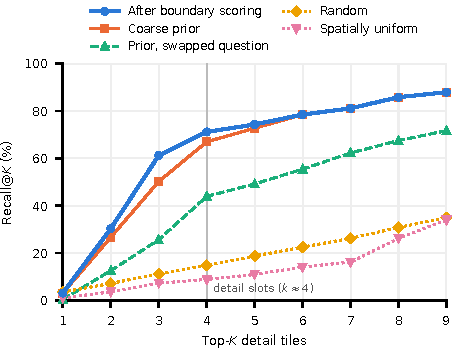
\includegraphics[width=\linewidth]{figures/fig_recall.pdf}
  \caption{\textbf{Reliability of low-resolution attention} on V$^*$~Bench ($B=1536$). Recall@$K$ is the
  fraction of questions whose target is covered by the top $K$ detail tiles. Swapped question: the prior
  computed with the question of another image of the same category.}
  \label{fig:recall}
\end{figure}

\paragraph{The prior can filter.}
With the top four of a median of 24 tiles, the coarse prior covers the target on 67.0\% of the questions, against
14.8\% for random and 8.9\% for spatially uniform selection (\cref{fig:recall}). It also follows the question:
with the question of another image, recall drops to 44.0\%, by 23.0 points (95\% CI [15.7, 30.9]).

\paragraph{The decision needs high resolution.}
The first-ranked tile of the prior covers the target on only 3.1\% of the questions. At the same $K$, boundary
scoring raises recall at every budget, from 27.7\% to 69.1\% at $B=1024$ and from 67.0\% to 71.2\% at
$B=1536$, and it recovers 64 to 90\% of the targets in the window that the prior alone would miss
(\cref{tab:recall,tab:window}). This recall is not the final accuracy, which \cref{sec:main} reports.

% ─────────────────────────────────────────────────────────────────────────────
\subsection{Motivation}
\label{sec:design}

These observations motivate three design choices of \method: since cost arises when tiles are computed, the
decision is made before the vision encoder and the KV cache is built by streaming; since low-resolution
attention finds candidates for the question, the VLM's own attention over a low-resolution view filters the
tiles, without any other model; and since the final choice needs high resolution only near the cut-off, only
a small boundary window is encoded and scored.

\paragraph{Problem setting.}
Given a budget of $B$ visual tokens, \ie $K=\lfloor B/n\rfloor$ tiles, we want to choose \emph{before
encoding} which tiles to keep, such that the vision encoder, the language model, and the KV cache
each process $\mathcal{O}(K)$ tokens independently of $N$.

% ─────────────────────────────────────────────────────────────────────────────
% Sec. 4  Method (preliminaries moved to 3_motivation.tex). Every number here matches foveatile_internvl.py / foveatile_config.py (frozen v1.0).
% ─────────────────────────────────────────────────────────────────────────────
\section{Method}
\label{sec:method}

\method decides \emph{which} image regions to encode before any of them reaches the vision encoder.
It keeps a low-resolution view of the whole image, uses the VLM itself to rank the high-resolution tiles
by their relevance to the question, and streams only the selected tiles into the KV cache. \cref{fig:method} gives an overview; the supplementary material lists the entire procedure (\cref{alg:foveatile}).

\begin{figure*}[t]
  \centering
  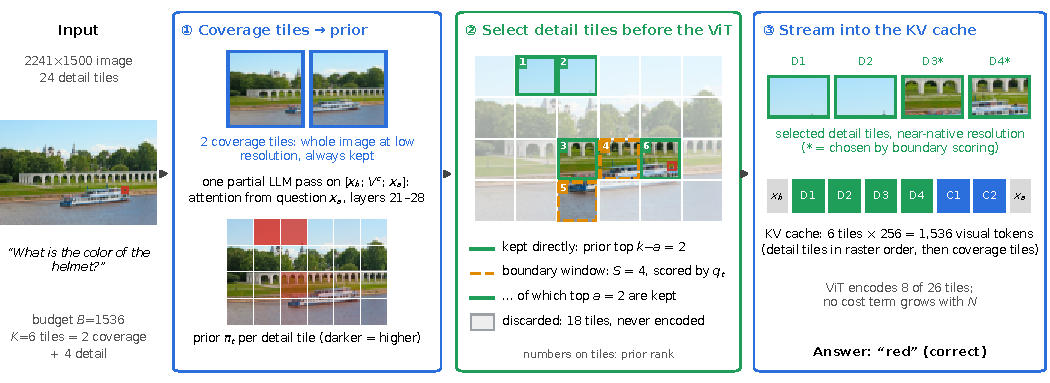
\includegraphics[width=\linewidth]{figures/fig_overview.pdf}
  \caption{\textbf{Overview of \method.} The image is represented at two scales: $m$ coverage tiles
  that show the whole image at low resolution, and a grid of $N$ detail tiles at near-native resolution.
  A single partial forward pass over the coverage tiles yields a question-aware prior over the detail
  tiles. The top-ranked tiles are kept directly, the tiles at the selection boundary are re-scored with
  question attention, and all other tiles are discarded \emph{before} the vision encoder. The selected
  tiles are streamed into the KV cache, so compute and memory are bounded by the budget $K$ rather than
  by $N$. Example from V$^*$~Bench~\cite{vstar} with $B=1536$ ($K=6$); the 3:2 image fits a $2\times1$ coverage grid, so the
  spare slot goes to the detail tiles. The prior ranks the target tile only sixth, and boundary scoring
  recovers it.}
  \label{fig:method}
\end{figure*}

% ─────────────────────────────────────────────────────────────────────────────
\subsection{Coverage tiles and detail tiles}
\label{sec:scales}

\method represents the image at two scales and splits the $K$ tile slots between them.

\paragraph{Coverage tiles.} The whole image is resized to a $c_c\times r_c$ grid of at most $m$ tiles,
where $m=\max(1,\lfloor K/2\rfloor)$. The official tiling optimizes only the aspect-ratio match and
often leaves part of such a budget unused. We instead pick the grid with the \emph{most} tiles,
$c_c r_c\le m$, among those whose aspect-ratio distortion is at most $1.75\times$, so that the coverage
tiles use their share of the budget. The coverage tiles are always kept. They give the model the global layout
and context of the image, and they are the input to the prior (\cref{sec:prior}).

\paragraph{Detail tiles.} The detail tiles are the official $c\times r$ grid with $N\le N_{\max}=47$
tiles, \ie close to native resolution. \method keeps $k=K-c_cr_c$ of them, so slots that the coverage grid
cannot fill go to detail tiles.

With $m=1$, the coverage tile reduces to the official thumbnail; the even split between the two scales
is calibrated (\cref{sec:impl}).

% ─────────────────────────────────────────────────────────────────────────────
\subsection{Question-aware prior from coverage tiles}
\label{sec:prior}

To rank the detail tiles without encoding them, we ask the VLM where it looks when it reads the question
against the low-resolution view. This builds on the observation that VLMs attend to the relevant region
even when they cannot resolve its details~\cite{vicrop}, which we quantified in \cref{sec:reliability}. We compute a single prior from the coverage
tiles, before any detail tile is encoded: we run the language
model on
$[\,\mathbf{x}_b;\ \mathbf{V}^{c};\ \mathbf{x}_a\,]$, where $\mathbf{V}^{c}\in\mathbb{R}^{nm\times d}$
are the coverage tokens, and stop after layer $l_{\text{hi}}$. Let $\mathbf{A}^{(l)}$ be the
head-averaged attention of layer $l$. The saliency of coverage patch $j$ is the attention it receives
from all text positions after the image, averaged over a band of middle-to-late layers
$\mathcal{L}_p=\{l_{\text{lo}},\dots,l_{\text{hi}}\}$, where visual information is transferred to the
question tokens~\cite{crossmodalflow}:
\begin{equation}
  s_j=\frac{1}{|\mathcal{L}_p|}\sum_{l\in\mathcal{L}_p}\frac{1}{|\mathbf{x}_a|}
      \sum_{i\in\mathbf{x}_a}\mathbf{A}^{(l)}_{i,j}.
  \label{eq:saliency}
\end{equation}
After min-max normalization, each coverage patch is assigned to the detail tile that contains its
center in normalized image coordinates, and the prior of detail tile $t$ is the mean saliency of its
patches, $\pi_t=\frac{1}{|P_t|}\sum_{j\in P_t}s_j$, again min-max normalized.

This pass costs a single forward over $|\mathbf{x}_b|+nm+|\mathbf{x}_a|$ tokens through
$l_{\text{hi}}$ of the $L$ layers, which is independent of $N$. We compute only the attention rows of
$\mathbf{x}_a$ in \cref{eq:saliency} and keep the fused attention kernel for the forward pass, so the
full attention matrix is never materialized. The pass also produces the KV cache of the prefix
$[\,\mathbf{x}_b;\ \mathbf{V}^{c}\,]$, which the next stage reuses.

% ─────────────────────────────────────────────────────────────────────────────
\subsection{Boundary scoring with question attention}
\label{sec:boundary}

The prior is computed at low resolution, so it can bring the target close to the top of the ranking but
cannot make the final choice on its own (\cref{sec:reliability}). \method therefore spends additional computation only on the tiles at the selection
boundary (\cref{fig:boundary}), similar to retrieve-then-rerank pipelines that apply an expensive scorer
only to the candidates of a cheap first stage~\cite{monobert}. Let the detail tiles be sorted by $\pi_t$, let $k$ be the number of
detail slots, and let $S$ be the size of the scoring window. With $a=\min(k,\lfloor S/2\rfloor)$, the top $k-a$ tiles are \emph{kept
directly} (encoded, not scored), the next $S$ tiles form the \emph{boundary window}, which is encoded and
scored and whose $a$ highest-scoring tiles are kept, and all remaining tiles are \emph{discarded} and never
reach the vision encoder.
The score of a boundary tile $t$ is its question attention at layer $l_q$, measured in the context of
the coverage tiles:
\begin{equation}
  q_t=\frac{1}{|\mathbf{x}_a|}\sum_{i\in\mathbf{x}_a}\ \sum_{j\in\mathbf{V}_t}
      \mathbf{A}^{(l_q)}_{i,j}
  \quad\text{on}\quad [\,\mathbf{x}_b;\ \mathbf{V}^{c};\ \mathbf{V}_t;\ \mathbf{x}_a\,].
  \label{eq:qattn}
\end{equation}
Because the prefix $[\,\mathbf{x}_b;\ \mathbf{V}^{c}\,]$ is shared by all candidates, its keys and values
for layers $1,\dots,l_q$ are taken from the prior pass, as in prompt caching~\cite{promptcache}. Each candidate therefore costs one pass of
$n+|\mathbf{x}_a|$ tokens through $l_q$ layers, and this is mathematically identical to a full forward
over the sequence in \cref{eq:qattn}. Since $q_t$ depends only on tile $t$ and the question, the top-$a$
selection can be made on the fly with a size-$a$ min-heap while the window is streamed, without holding
all candidates in memory. Setting $S=0$ reduces \method to prior-only selection.


% ─────────────────────────────────────────────────────────────────────────────
\subsection{Streaming KV construction}
\label{sec:streaming}

\method builds the KV cache incrementally. It first prefills $\mathbf{x}_b$, then encodes the coverage
tiles and runs the prior. The candidate detail tiles, \ie the directly kept tiles and the boundary window,
are encoded in raster order in micro-batches of four tiles; boundary tiles are scored as they arrive and
enter or leave the size-$a$ pool. Once selection is final, the selected detail tiles are written to the
KV cache in raster order, followed by the $m$ coverage tiles. This mirrors the order seen in training,
where grid tiles precede the global thumbnail. The visual tokens are prefilled in chunks of 1{,}024
tokens with contiguous position ids after $\mathbf{x}_b$. Finally, $\mathbf{x}_a$ is prefilled and the
answer is decoded from the resulting cache of at most $|\mathbf{x}_b|+nK+|\mathbf{x}_a|$ tokens. The
visual tokens resident in memory never exceed about $k+m$ tiles plus one micro-batch, \ie
$\mathcal{O}(K)$.


\paragraph{Cost.}
\cref{tab:complexity} summarizes the cost per image. \method encodes $c_cr_c+(k-a)+S=K-a+S$ tiles. Its
language-model work consists of the prior pass over $|\mathbf{x}_b|+nm+|\mathbf{x}_a|$ tokens
($l_{\text{hi}}$ layers), $S$ scoring passes of $n+|\mathbf{x}_a|$ tokens ($l_q$ layers), and the main
prefill of $nK$ visual tokens. Every term depends on the budget $K$ and the window $S$, but none depends
on the number of tiles $N$ (per-stage timings in \cref{tab:ttft}). The KV cache is bounded by the budget. In contrast, every method that prunes
after encoding pays $\mathcal{O}(N)$ vision compute, and methods that prune inside the language model
also pay $\mathcal{O}(N)$ in the layers before pruning.

\begin{table}[t]
  \centering
  \small
  \setlength{\tabcolsep}{4pt}
  \begin{tabular}{lccc}
    \toprule
    Method & ViT & LLM prefill & KV cache \\
    \midrule
    Uncompressed & $N$ & $N$ & $N$ \\
    VisionZip, HiRED & $N$ & $K$ & $K$ \\
    FastV, SparseVLM & $N$ & $N\!\to\!K$ & $\approx K$ \\
    IF-Prune & $N^{\ddagger}$ & $N\!\to\!K$ & $\approx K$ \\
    \method (ours) & $K{-}a{+}S$ & $K{+}m{+}S^{\dagger}$ & $K$ \\
    \bottomrule
  \end{tabular}
  \caption{\textbf{Cost per image} in units of tiles ($n=256$ tokens each), with $N$ detail tiles and a
  budget of $K$ tiles; text tokens are omitted. $N\!\to\!K$: all $N$ tiles pass through the layers
  before pruning, $K$ remain after. $^{\ddagger}$Plus a 1B guide VLM on all $N$ tiles.
  $^{\dagger}$The $m$ coverage and $S$ boundary tiles pass only through the first $l_{\text{hi}}$ and
  $l_q$ layers. Only \method is independent of $N$.}
  \label{tab:complexity}
\end{table}

% ─────────────────────────────────────────────────────────────────────────────
\subsection{Hyperparameters and calibration}
\label{sec:impl}

\method has no trained parameters. The coverage fraction $m/K$, the window $S$ for each budget, and the default
budget are set once on held-out data and frozen for all test sets: 600 questions from the InfoVQA \emph{train}
split and 600 from MME-RealWorld outside its Lite subset and images, which share no questions or images with any
test set. On these sets, $m/K=0.5$ is within 0.1 points of the best average accuracy and has the most stable
worst-task accuracy, whereas the thumbnail alone ($m=1$) is about 7 points lower (\cref{tab:ablation}). Without
boundary scoring ($S=0$), remote sensing questions lose up to 10.8 raw points, while windows up to four times
larger give no reliable gain, so we use $S=\{5,4,4,3,3\}$ for $B=\{1024,1536,2048,2560,3072\}$. The default
$B=1536$ ($K=6$, $m=3$, $S=4$) is where held-out accuracy saturates. The attention layers,
$\mathcal{L}_p=\{21,\dots,28\}$ and $l_q=20$ for InternVL3.5-8B ($L=36$), were fixed in preliminary experiments
before this protocol. The full protocol, including deviations from our pre-registered rules, is in the
supplementary material.

% NOTE: L_p and l_q were chosen on InfoVQA val before the held-out protocol existed
% (docs/04_calibration_protocol.md, 1.8.3 note). Disclose this in the supplementary.

% ─────────────────────────────────────────────────────────────────────────────
% Sec. 5  Experiments. Tables / figures are generated by results/paper/build_paper_results.py
% (re-run it after new results arrive; cells still missing print as a red "?").
% Needs in preamble.tex: \usepackage{multirow} \usepackage{colortbl} \definecolor{oursbg}{HTML}{E8F0FC}
% ─────────────────────────────────────────────────────────────────────────────
\section{Experiments}
\label{sec:exp}

Our central claim is that the memory and latency of \method do not grow with the input resolution,
while its accuracy matches the strongest token-pruning methods. \cref{sec:main} compares accuracy under
memory and token budgets, \cref{sec:scaling} varies the resolution, and \cref{sec:ablation} studies the
components of \method.

\providecommand{\pend}{\textcolor{red}{?}}

\begin{table*}[t]
  \centering
  \footnotesize
  \setlength{\tabcolsep}{4pt}
  \begin{tabular}{l cc c cc c ccc}
    \toprule
    & \multicolumn{2}{c}{Document} & Real-world & \multicolumn{2}{c}{High resolution} & & \multicolumn{3}{c}{Saving \vs uncompressed$\uparrow$} \\
    \cmidrule(lr){2-3}\cmidrule(lr){4-4}\cmidrule(lr){5-6}\cmidrule(lr){8-10}
    Method & DocVQA & InfoVQA & MME-RW & HR-Bench 4K & V$^*$ Bench & Avg.\ (\%) & TTFT & Memory & FLOPs \\
    \midrule
    \multicolumn{10}{c}{\textit{Upper bound: all visual tokens}} \\
    Uncompressed & 91.4 & 78.7 & 51.6 & 62.0 & 83.8 & 100.0 & 1.0$\times$ & 1.0$\times$ & 1.0$\times$ \\
    \midrule
    \multicolumn{10}{c}{\textit{Budget $B=1536$ visual tokens (default), $\approx$21\% of all visual tokens}} \\
    FastV~\cite{fastv} & 84.0 & 61.0 & 46.9 & \underline{59.0} & 79.1 & 90.0 & 2.5$\times$ & 1.5$\times$ & 2.9$\times$ \\
    SparseVLM~\cite{sparsevlm} & 55.1 & 62.2 & \underline{50.2} & \textbf{59.5} & \underline{79.6} & 85.5 & 2.2$\times$ & 1.5$\times$ & 2.4$\times$ \\
    VisionZip~\cite{visionzip} & 48.7 & 47.6 & 41.7 & 49.0 & 70.2 & 71.5 & \underline{2.7$\times$} & \underline{4.2$\times$} & \underline{3.2$\times$} \\
    HiRED~\cite{hired} & 58.5 & 51.6 & 45.2 & 53.5 & 72.8 & 78.0 & \textbf{2.8$\times$} & 3.7$\times$ & \textbf{3.3$\times$} \\
    IF-Prune~\cite{ifprune} & \textbf{88.2} & \underline{72.7} & 49.3 & 57.5 & \textbf{81.7} & \underline{94.9} & 1.5$\times$ & 0.7$\times$ & 1.8$\times$ \\
    \rowcolor{oursbg}
    \method (ours) & \underline{87.0}$^{\downarrow}$ & \textbf{74.8}$^{\uparrow}$ & \textbf{52.1}$^{\uparrow}$ & 56.5 & 77.5 & \textbf{95.0} & 2.4$\times$ & \textbf{5.0$\times$} & \underline{3.2$\times$} \\
    \midrule
    \multicolumn{10}{c}{\textit{Budget $B=2560$ visual tokens, $\approx$35\% of all visual tokens}} \\
    FastV~\cite{fastv} & \underline{89.6} & 70.5 & 50.1 & \underline{59.0} & \underline{81.7} & 95.5 & 2.0$\times$ & 1.5$\times$ & 2.2$\times$ \\
    SparseVLM~\cite{sparsevlm} & 69.8 & 71.1 & \underline{51.8} & 57.0 & 81.2 & 91.2 & 1.7$\times$ & 1.4$\times$ & 1.8$\times$ \\
    VisionZip~\cite{visionzip} & 62.8 & 57.9 & 45.9 & 57.5 & 76.4 & 83.0 & \underline{2.1$\times$} & \underline{2.8$\times$} & \underline{2.4$\times$} \\
    HiRED~\cite{hired} & 67.8 & 59.2 & 48.2 & 58.0 & 77.5 & 85.8 & \textbf{2.2$\times$} & 2.6$\times$ & \textbf{2.5$\times$} \\
    IF-Prune~\cite{ifprune} & \underline{89.6} & \underline{74.8} & 49.9 & \textbf{59.5} & \textbf{83.8} & \underline{97.1} & 1.3$\times$ & 0.7$\times$ & 1.5$\times$ \\
    \rowcolor{oursbg}
    \method (ours) & \textbf{90.1} & \textbf{78.6}$^{\uparrow}$ & \textbf{52.2} & 58.0 & 79.6 & \textbf{97.6} & 1.7$\times$ & \textbf{3.6$\times$} & 2.2$\times$ \\
    \midrule
    \multicolumn{10}{c}{\textit{Budget $B=3072$ visual tokens, $\approx$42\% of all visual tokens}} \\
    FastV~\cite{fastv} & \textbf{90.8} & 73.6 & 49.7 & \textbf{61.0} & \underline{82.7} & 97.2 & \underline{1.8$\times$} & 1.5$\times$ & \underline{2.0$\times$} \\
    SparseVLM~\cite{sparsevlm} & 69.8 & 72.5 & \underline{51.0} & 57.0 & \textbf{83.8} & 91.8 & 1.5$\times$ & 1.3$\times$ & 1.6$\times$ \\
    VisionZip~\cite{visionzip} & 68.8 & 61.8 & 47.4 & 56.5 & 78.5 & 86.1 & \textbf{1.9$\times$} & \underline{2.4$\times$} & \textbf{2.2$\times$} \\
    HiRED~\cite{hired} & 71.1 & 61.8 & 49.2 & \underline{60.0} & 81.7 & 89.2 & \textbf{1.9$\times$} & 2.3$\times$ & \textbf{2.2$\times$} \\
    IF-Prune~\cite{ifprune} & 90.1 & \underline{75.1} & 49.8 & \textbf{61.0} & 82.2 & \underline{97.4} & 1.2$\times$ & 0.7$\times$ & 1.4$\times$ \\
    \rowcolor{oursbg}
    \method (ours) & \underline{90.3} & \textbf{79.4}$^{\uparrow}$ & \textbf{53.5}$^{\uparrow}$ & 59.5 & 81.7 & \textbf{99.3} & 1.4$\times$ & \textbf{2.7$\times$} & 1.8$\times$ \\
    \bottomrule
  \end{tabular}
  \caption{\textbf{Accuracy and cost on InternVL3.5-8B.} Scores on each benchmark; Avg.\ is the mean percentage of the uncompressed score over the five benchmarks. HR-Bench 8K is in \cref{tab:hr8k}. Cost is the saving relative to the uncompressed model (higher is better), averaged over the five benchmarks. $^{\uparrow}$/$^{\downarrow}$: \method is significantly better/worse than the strongest baseline on that benchmark (paired bootstrap, 95\%); unmarked differences are not significant. Best compressed result per budget in \textbf{bold}, second \underline{underlined}.}
  \label{tab:main}
\end{table*}


% ─────────────────────────────────────────────────────────────────────────────
\subsection{Setup}
\label{sec:setup}

\paragraph{Models and benchmarks.}
We evaluate on InternVL3.5-4B, -8B, and -14B~\cite{internvl35}, and use the 8B model unless stated
otherwise. We cover three kinds of high-resolution inputs: documents (DocVQA val~\cite{docvqa}, 5,349
questions; InfoVQA val~\cite{infovqa}, 2,801), real-world scenes (MME-RealWorld Lite~\cite{mmerealworld},
1,919), and very high-resolution images with small targets (HR-Bench 4K and 8K~\cite{hrbench}, 800
questions each; V$^*$ Bench~\cite{vstar}, 191). We report ANLS on DocVQA and InfoVQA, CircularEval
accuracy on HR-Bench (a question counts only if all four option orders are answered correctly), and
multiple-choice accuracy otherwise. All methods use greedy decoding and the same prompts, and start
from the same official dynamic tiling with up to $N_{\max}=47$ tiles plus a thumbnail. Averages in
\cref{tab:main} are over the first five benchmarks; HR-Bench 8K is used for the resolution study of
\cref{sec:scaling}.

\paragraph{Baselines.}
We compare with FastV~\cite{fastv}, SparseVLM~\cite{sparsevlm}, VisionZip~\cite{visionzip}, and
IF-Prune~\cite{ifprune}, ported to InternVL3.5 from the official code with the official
hyperparameters: FastV and IF-Prune prune at layer 2, IF-Prune uses the released InternVL2.5-1B guide
model, SparseVLM prunes at the official relative depths with its pruning rate calibrated per budget,
and VisionZip keeps dominant and contextual tokens in each tile. For all methods, the budget $B$ is the
number of visual tokens left in the KV cache. We also compare with two same-budget downscaling baselines
(\cref{sec:downscale}). Implementation details are in the supplementary material.

\paragraph{Efficiency measurement.}
All measurements use one NVIDIA A6000 (48\,GB), bfloat16, and batch size 1. TTFT is the wall-clock time
to the first generated token, including the vision encoder and any scoring or guide model, and we report the median over 50 images per benchmark after one warm-up image. Memory is the peak
allocated GPU memory minus the model weights; for IF-Prune it includes the guide model. FLOPs count the
vision encoder and the prefill up to the first token.

\paragraph{Protocol.}
All \method hyperparameters are fixed on held-out calibration data (\cref{sec:impl}), except for the attention layers, which were chosen in preliminary experiments and are disclosed in the supplementary material; no test set is used for any other choice. We test differences with a paired bootstrap over questions (or CircularEval groups) at
95\% confidence.

% ─────────────────────────────────────────────────────────────────────────────
\subsection{Accuracy under a memory budget}
\label{sec:main}

\providecommand{\pend}{\textcolor{red}{?}}

\begin{table}[t]
  \centering
  \footnotesize
  \setlength{\tabcolsep}{2.2pt}
  \begin{tabular}{l cccc}
    \toprule
    & \multicolumn{4}{c}{Memory limit per image} \\
    \cmidrule(lr){2-5}
    Method & $\leq$0.5\,GB & $\leq$1\,GB & $\leq$2\,GB$^\dagger$ & None \\
    \midrule
    FastV & -- & -- & \underline{97.2}\,{\tiny (3072)} & 97.2\,{\tiny (3072)} \\
    SparseVLM & -- & -- & 91.8\,{\tiny (3072)} & 91.8\,{\tiny (3072)} \\
    VisionZip & 71.5\,{\tiny (1536)} & 86.1\,{\tiny (3072)} & 86.1\,{\tiny (3072)} & 86.1\,{\tiny (3072)} \\
    HiRED & \underline{72.3}\,{\tiny (1024)} & \underline{89.2}\,{\tiny (3072)} & 89.2\,{\tiny (3072)} & 89.2\,{\tiny (3072)} \\
    IF-Prune & -- & -- & -- & \underline{97.4}\,{\tiny (3072)} \\
    \rowcolor{oursbg}
    \method (ours) & \textbf{95.0}\,{\tiny (1536)} & \textbf{99.3}\,{\tiny (3072)} & \textbf{99.3}\,{\tiny (3072)} & \textbf{99.3}\,{\tiny (3072)} \\
    \bottomrule
  \end{tabular}
  \caption{\textbf{Accuracy under a memory limit} on InternVL3.5-8B: the best mean percentage of the uncompressed score (five benchmarks of \cref{tab:main}) that each method reaches with budgets $B\in\{1024,\dots,3072\}$ while its peak memory on top of the model weights stays within the limit (budget in parentheses; --: no budget fits; $^\dagger$the memory of the uncompressed model). FastV, SparseVLM, and IF-Prune need at least 1.3\,GB at any budget, and IF-Prune needs more memory than the uncompressed model.}
  \label{tab:memcap}
\end{table}


The number of high-resolution requests a GPU can serve is bounded by memory, so we first ask which
accuracy each method reaches within a memory limit (\cref{tab:memcap}). \method is the most accurate
method under every limit. Within 1\,GB per image, it retains 99.3\% of the uncompressed accuracy, while
FastV, SparseVLM, and IF-Prune cannot run at any budget, and VisionZip reaches 86.1\%. IF-Prune even needs
more memory than the uncompressed model (3.0 \vs 2.0\,GB), mainly for its guide model, so it does not fit
within the uncompressed model's own footprint. Without a limit, \method still has the highest accuracy
(99.3\% at $B=3072$).

\cref{tab:main} compares all methods at equal token budgets. At the default budget $B=1536$, which keeps
about a fifth of the visual tokens, \method retains 95.0\% of the uncompressed accuracy on average, the
highest of all methods, ahead of IF-Prune (94.9\%), FastV (90.0\%), SparseVLM (85.5\%), and VisionZip
(71.5\%). It needs 5.0$\times$ less memory than the uncompressed model, against 1.5$\times$ for FastV and SparseVLM and
0.7$\times$ for IF-Prune, and it is 1.6$\times$ faster than IF-Prune. From $B=1536$ upward,
\method has the highest average accuracy of all methods at every budget, reaching 99.3\% at $B=3072$,
while using the least memory.

\method is strongest where the answer depends on the layout of the whole image. On InfoVQA it is
significantly better than every baseline at every budget, by 2.1 to 4.3 points over the strongest one,
and on MME-RealWorld it even exceeds the uncompressed model (significantly at $B=3072$, +1.9 points):
its high-resolution scenes contain large regions irrelevant to the question, and keeping only the
coverage view and the question-relevant tiles removes these distractors, which may also explain why more
tiles lower the accuracy of the uncompressed model on HR-Bench 8K (\cref{tab:hr8k}). On HR-Bench and V$^*$ Bench, which ask about
small objects, \method is within a few points of the best baseline, and none of these differences is
significant at any budget.

\begin{figure}[t]
  \centering
  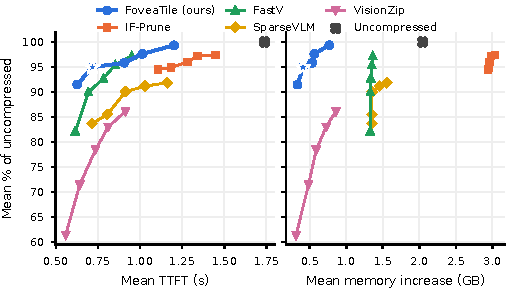
\includegraphics[width=\linewidth]{figures/fig_pareto.pdf}
  \caption{\textbf{Accuracy--cost trade-off} on InternVL3.5-8B, averaged over the five benchmarks of \cref{tab:main}, for
  $B\in\{1024,1536,2048,2560,3072\}$. The star marks the default \method budget. \method uses the least
  memory at every budget, and every configuration of IF-Prune and SparseVLM is dominated by a \method
  configuration that is both faster and more accurate.}
  \label{fig:pareto}
\end{figure}

\cref{fig:pareto} shows the full trade-off over five budgets. In memory, \method has the best curve at every budget: even its largest budget uses less memory than any budget of FastV, SparseVLM,
or IF-Prune. In TTFT, \method reaches the highest accuracy of all methods (99.3\% at 1.2\,s), and every
configuration of IF-Prune and SparseVLM is dominated by a \method configuration that is both faster and
more accurate: at about the same TTFT as IF-Prune at $B=1536$ (1.2\,s), \method reaches 99.3\% instead
of 94.9\%, and at $B=1536$ (95.0\%) it is more accurate than IF-Prune at any $B\leq1536$ with about
0.6$\times$ its TTFT and one seventh of its memory.

\begin{table}[t]
  \centering
  \footnotesize
  \setlength{\tabcolsep}{3.4pt}
  \begin{tabular}{l cc cc cc}
    \toprule
    & \multicolumn{2}{c}{$B=1536$} & \multicolumn{2}{c}{$B=2560$} & \multicolumn{2}{c}{$B=3072$} \\
    \cmidrule(lr){2-3}\cmidrule(lr){4-5}\cmidrule(lr){6-7}
    Method & Avg. & Small & Avg. & Small & Avg. & Small \\
    \midrule
    Low-Res & 84.2 & 73.5 & 92.9 & 85.4 & 93.3 & 85.9 \\
    Low-Res-Fill & 91.7 & 82.6 & 94.1 & 86.6 & 96.2 & 90.3 \\
    \rowcolor{oursbg}
    \method (ours) & \textbf{95.0} & \textbf{91.9} & \textbf{97.6} & \textbf{93.8} & \textbf{99.3} & \textbf{95.5} \\
    \bottomrule
  \end{tabular}
  \caption{\textbf{Same-budget downscaling}, as a percentage of the uncompressed score. Avg.: the five benchmarks of \cref{tab:main}; Small: HR-Bench 4K, HR-Bench 8K, and V$^*$. Low-Res is the official tiling capped at $K=B/256$ tiles, which cannot always fill the budget (on average 1{,}149/1{,}931/1{,}972 visual tokens); Low-Res-Fill gives the whole budget to coverage tiles ($m{=}K$). Per-benchmark scores and paired confidence intervals are in the supplementary material.}
  \label{tab:downscale}
\end{table}


\paragraph{Same-budget downscaling.}
\label{sec:downscale}
A simpler way to meet the budget is to downscale the image. We test two versions at the same $B$: the
official tiling capped at $K=B/256$ tiles (Low-Res), and the coverage tiles of \method given the whole
budget ($m{=}K$, Low-Res-Fill). \method retains more of the uncompressed accuracy at every budget
(95.0/97.6/99.3\% \vs 91.7/94.1/96.2\% for Low-Res-Fill, \cref{tab:downscale}), and the gap is largest on
the small-object benchmarks (91.9/93.8/95.5\% \vs 82.6/86.6/90.3\%). On HR-Bench and V$^*$ Bench, \method is
ahead of Low-Res-Fill in all nine comparisons, by 2.5 to 8.0 points, significantly on HR-Bench 8K at
$B=1536$; on MME-RealWorld it is significantly better at every budget. Spending part of the budget on
question-relevant detail tiles is thus better than spending all of it on a uniformly sharper view.

\paragraph{Model scale.}
With the hyperparameters calibrated on the 8B model, \method reaches 94.5\% and 95.2\% on InternVL3.5-4B
and \mbox{-14B} at $B=1536$, with peak memory of 0.37 and 0.43\,GB, about 7$\times$ less than IF-Prune. The full
table is in the supplementary material.

% ─────────────────────────────────────────────────────────────────────────────
\subsection{Memory and latency that do not grow with resolution}
\label{sec:scaling}

\begin{figure}[t]
  \centering
  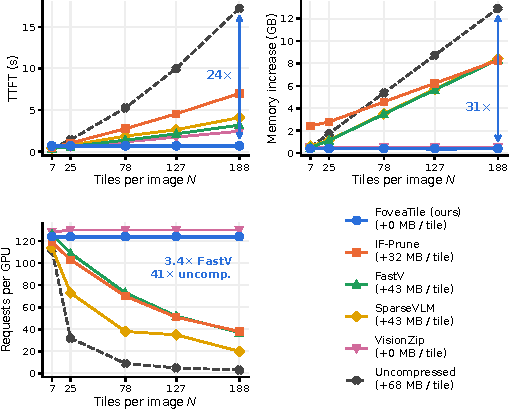
\includegraphics[width=\linewidth]{figures/fig_scaling.pdf}
  \caption{\textbf{Cost as the input resolution grows} (HR-Bench 8K, $B=1536$; the tile cap is raised so
  that the same images split into 7 to 188 tiles). The legend gives the growth of peak memory per added
  tile. \method stays flat in TTFT, memory, and requests per GPU, while every method that prunes inside
  the language model degrades with $N$.}
  \label{fig:scaling}
\end{figure}

\providecommand{\pend}{\textcolor{red}{?}}

\begin{table}[t]
  \centering
  \footnotesize
  \setlength{\tabcolsep}{3.2pt}
  \begin{tabular}{l ccc ccc}
    \toprule
    & \multicolumn{3}{c}{25 tiles} & \multicolumn{3}{c}{188 tiles} \\
    \cmidrule(lr){2-4}\cmidrule(lr){5-7}
    Method & Acc. & TTFT & Mem. & Acc. & TTFT & Mem. \\
    \midrule
    Uncompressed & 56.5 & 1.44 & 1.79 & 49.0 & 17.22 & 12.90 \\
    \midrule
    FastV & \textbf{54.0} & 0.63 & 1.16 & 42.5 & 3.19 & 8.34 \\
    SparseVLM & 53.5 & 0.76 & 1.18 & 51.5 & 4.09 & 8.44 \\
    VisionZip & 44.5 & \textbf{0.58} & 0.49 & 27.0 & 2.45 & 0.49 \\
    HiRED & 48.5 & \textbf{0.58} & 0.54 & 41.0 & 2.35 & 0.88 \\
    IF-Prune & 52.5 & 1.04 & 2.81 & \textbf{52.0} & 7.00 & 8.28 \\
    \rowcolor{oursbg}
    \method (ours) & 52.0 & 0.70 & \textbf{0.42} & 47.0 & \textbf{0.71} & \textbf{0.41} \\
    \bottomrule
  \end{tabular}
  \caption{\textbf{Higher input resolution at a fixed budget} ($B=1536$) on HR-Bench 8K. Raising the tile cap from $N_{\max}=47$ to 200 splits each image into 188 tiles instead of about 25. Acc.\ is CircularEval accuracy, TTFT in seconds, Mem.\ in GB.}
  \label{tab:hr8k}
\end{table}


To isolate the effect of resolution, we raise the tile cap on HR-Bench 8K so that the same images are
split into 7 to 188 tiles, and measure cost at $B=1536$ (\cref{fig:scaling}). The peak memory of \method
does not grow at all: it stays at 0.41\,GB from 7 to 188 tiles, because no stage of \method ever holds
more than the budget. Every method that prunes inside the language model grows linearly with $N$, by
32 to 43\,MB per added tile (68\,MB for the uncompressed model), and needs over 8\,GB at 188 tiles,
20$\times$ more than \method. TTFT behaves the same way: \method stays at 0.7\,s, whereas FastV and
IF-Prune become 4.5$\times$ and 10$\times$ slower than \method at 188 tiles, and the uncompressed model
24$\times$ slower. VisionZip also keeps its memory flat, since it prunes before the language model, but
it still encodes every tile, so its TTFT grows with $N$, and its accuracy is 23.5 points lower on average
(\cref{tab:main}). \method is the only method whose memory and latency are both independent of the
resolution. Beyond about 35 tiles, \method is the fastest of all methods, and its lead grows with
$N$.

Memory determines how many requests a GPU can serve. We measure this directly: on one A6000 (33\,GB free
after the 8B weights), we prefill requests one after another, keep the KV cache of each, as if it were
still decoding, and count the requests that complete before the GPU runs out of memory. \method holds 124
requests at every resolution, from 7 to 188 tiles. With FastV and IF-Prune this number falls from 103--109
at 25 tiles to 37--38 at 188 tiles, with SparseVLM to 20, and with the uncompressed model from 32 to 3. At
188 tiles, \method serves 3.4$\times$ more requests than FastV, 3.3$\times$ more than IF-Prune,
6.2$\times$ more than SparseVLM, and 41$\times$ more than the uncompressed model.

\cref{tab:hr8k} reports accuracy at both resolutions. Splitting the image more finely at a fixed budget
lowers accuracy for every method, and even for the uncompressed model (56.5 to 49.0). Among the
compressed methods, \method has the best accuracy per unit cost: at 188 tiles it is 10$\times$ faster
than IF-Prune and 6$\times$ faster than SparseVLM with 20$\times$ less memory, and it is more accurate
than FastV (47.0 \vs 42.5) at 4.5$\times$ less TTFT. With a larger budget
($B=2560$), \method matches the best compressed methods at 188 tiles (52.5) and exceeds the uncompressed
model (49.0), which may suffer from the very long visual sequence.

% ─────────────────────────────────────────────────────────────────────────────
\subsection{Ablations}
\label{sec:ablation}

\providecommand{\pend}{\textcolor{red}{?}}

\begin{table}[t]
  \centering
  \footnotesize
  \setlength{\tabcolsep}{2.6pt}
  \begin{tabular}{l ccc cc c}
    \toprule
    Variant & Info & MME & Local & Avg. & Worst & TTFT \\
    \midrule
    \rowcolor{oursbg}
    \method & 94.4 & 97.1 & 100.1 & 95.8 & 85.4 & 0.92 \\
    Coverage only, $m{=}K$ & 95.8 & 95.6 & 95.8 & 95.7 & 77.5 & 0.58 \\
    Thumbnail, $m{=}1$ & 86.6 & 90.8 & 95.6 & 88.7 & 75.7 & -- \\
    Prior only, $S{=}0$ & 94.5 & 93.6 & 92.6 & 94.1 & 78.5 & 0.73 \\
    Window $2\times$ & 94.2 & 97.6 & 98.4 & 95.9 & 85.0 & 1.11 \\
    Window $4\times$ & 94.5 & 96.6 & 97.0 & 95.5 & 80.9 & 1.48 \\
    Random prior & 85.9 & 87.7 & 90.2 & 86.8 & 70.6 & -- \\
    \bottomrule
  \end{tabular}
  \caption{\textbf{Ablations} on the held-out calibration sets of \cref{sec:impl} (Info, MME), as a percentage of the uncompressed score. Local: MME-RealWorld remote sensing, monitoring, and autonomous driving. Worst: lowest percentage among InfoVQA and the five MME-RealWorld subtasks. Window sizes are relative to the default $S$; TTFT in seconds.}
  \label{tab:ablation}
\end{table}


\cref{tab:ablation} ablates the components of \method on the held-out calibration sets, averaged over
five budgets. Using the thumbnail alone as coverage ($m=1$) loses 7.1 points on average, so giving
the coverage tiles half of the budget is essential. Using only coverage tiles ($m=K$) gives the same average
as \method at lower TTFT, but its worst task drops from 85.4\% to 77.5\% and the local-detail subtasks
from 100.1\% to 95.8\%: detail tiles do not raise the average, they prevent failures on questions about
small regions. On the test sets, the same variant trails \method by 3.1 to 3.5 points in average retention
(Low-Res-Fill in \cref{tab:downscale}). Removing boundary scoring ($S=0$) costs 1.7 points on average, 6.9 on the worst task, and
7.5 on local-detail questions, so ranking by the prior alone is not enough. Larger windows add TTFT
without improving accuracy. Finally, replacing the question-aware prior with a random ranking, while
keeping boundary scoring, costs 9.0 points on average and 14.8 on the worst task: which detail tiles reach
the window matters most, and the attention of the VLM over the coverage tiles is what finds them. These accuracy results complement the
recall analysis of \cref{sec:reliability}.

% ─────────────────────────────────────────────────────────────────────────────
% Sec. 6  Conclusion.
% ─────────────────────────────────────────────────────────────────────────────
\section{Conclusion}
\label{sec:conclusion}

We presented \method, a training-free method that bounds the memory of high-resolution VLMs by
deciding which tiles to encode before the vision encoder, since token pruning removes tokens only after
they have been computed. On InternVL3.5, \method keeps 95.0\% of the uncompressed accuracy with
5.0$\times$ less memory and is the most accurate method under every memory limit. Its peak memory stays
constant from 7 to 188 tiles, so one GPU serves 41$\times$ more requests than the uncompressed model,
and its behavior carries over from 4B to 14B parameters without re-tuning.

\paragraph{Limitations.}
\method requires a VLM whose vision encoder processes each tile independently, so that the encoder can be
run on a subset of the tiles. All our experiments use InternVL3.5, but the same holds for other tile-based
VLMs: LLaVA-OneVision~\cite{llavaov}, for example, encodes each AnyRes crop separately and adds a
downscaled base image, so \method can be applied to it in the same way, although we have not evaluated it.
Native-resolution encoders~\cite{qwen2vl} attend across the whole image, so encoding only the selected
regions would change the input they were trained on; \method does not cover them.

Improving the recall of the prior for very small objects, evaluating other tile-based VLMs, and
extending the selection to native-resolution encoders and to video are directions for future work.

\section*{LLM Usage Statement}
We used Claude Code (Anthropic) to help write and run experiment code, analyze results, generate tables
and figures, and draft and edit the text of this paper, under the direction of the authors. The authors
reviewed these outputs and take responsibility for all content.

{
    \small
    \bibliographystyle{ieeenat_fullname}
    \bibliography{main}
}

% WARNING: do not forget to delete the supplementary pages from your submission
\clearpage
\setcounter{page}{1}
\renewcommand{\thepage}{S\arabic{page}}
\setcounter{section}{0}
\setcounter{table}{0}
\setcounter{figure}{0}
\setcounter{algorithm}{0}
\renewcommand{\thesection}{S\arabic{section}}
\renewcommand{\thetable}{S\arabic{table}}
\renewcommand{\thefigure}{S\arabic{figure}}
\renewcommand{\thealgorithm}{S\arabic{algorithm}}
\renewcommand{\theHsection}{S\arabic{section}}
\renewcommand{\theHtable}{S\arabic{table}}
\renewcommand{\theHfigure}{S\arabic{figure}}
\renewcommand{\theHalgorithm}{S\arabic{algorithm}}
% Top-align full-width tables on float pages instead of centering them vertically.
\makeatletter\setlength{\@dblfptop}{0pt}\makeatother
\maketitlesupplementary
% Column-width floats may stay where they are defined (the [t] of the shared table files would push them to the
% tops of later columns, away from their sections); full-width tables still go to the top of a page.
\let\origtable\table \let\endorigtable\endtable
\renewenvironment{table}[1][]{\origtable[!htbp]}{\endorigtable}
\let\origfigure\figure \let\endorigfigure\endfigure
\renewenvironment{figure}[1][]{\origfigure[!htbp]}{\endorigfigure}
\let\origalgorithm\algorithm \let\endorigalgorithm\endalgorithm
\renewenvironment{algorithm}[1][]{\origalgorithm[!htbp]}{\endorigalgorithm}
% ─────────────────────────────────────────────────────────────────────────────
% Supplementary: algorithm and boundary-scoring figure, moved from Sec. 4 for the page limit.
% ─────────────────────────────────────────────────────────────────────────────
\section{Procedure and boundary scoring}
\label{sec:supp_method}

\cref{alg:foveatile} lists the complete inference procedure of \method (\cref{sec:method}), and
\cref{fig:boundary} illustrates boundary scoring (\cref{sec:boundary}) on the example of \cref{fig:method}.

\begin{algorithm}[t]
\caption{\method inference for one question}
\label{alg:foveatile}
\begin{algorithmic}[1]
\Require image $I$, text $\mathbf{x}_b,\mathbf{x}_a$, budget $K$ tiles, window $S$
\State $m\gets\max(1,\lfloor K/2\rfloor)$
\State $k\gets K-c_cr_c$;\ \ $a\gets\min(k,\lfloor S/2\rfloor)$
\State $\mathcal{C}\gets$ KV cache after prefilling $\mathbf{x}_b$
\State $\mathbf{V}^{c}\gets\textsc{Encode}(\textsc{CoverageTiles}(I,m))$
\State $\pi,\ \mathcal{C}_{\text{pre}}\gets\textsc{Prior}(\mathbf{x}_b,\mathbf{V}^{c},\mathbf{x}_a)$
  \Comment{\cref{eq:saliency}, layers $\le l_{\text{hi}}$}
\State $\sigma\gets$ detail tiles of $I$ sorted by $\pi$ (descending)
\State $D\gets\sigma[1{:}k-a]$ \Comment{kept directly}
\State $W\gets\sigma[k-a+1{:}k-a+S]$ \Comment{rest: never encoded}
\State $\mathcal{H}\gets$ empty min-heap of capacity $a$
\For{each micro-batch $T\subset D\cup W$ in raster order}
  \State $\{\mathbf{V}_t\}_{t\in T}\gets\textsc{Encode}(T)$
  \For{$t\in T\cap W$}
    \State push $(q_t,\mathbf{V}_t)$ into $\mathcal{H}$ \Comment{\cref{eq:qattn}, reuses $\mathcal{C}_{\text{pre}}$}
    \If{$|\mathcal{H}|>a$} pop the lowest-scoring tile \EndIf
  \EndFor
\EndFor
\State $\mathcal{C}\gets\textsc{Prefill}(\mathcal{C},\ \text{tiles }D\cup\mathcal{H}\text{ in raster order},\ \mathbf{V}^{c})$
\State $\mathcal{C}\gets\textsc{Prefill}(\mathcal{C},\mathbf{x}_a)$;\ \ \Return $\textsc{Decode}(\mathcal{C})$
\end{algorithmic}
\end{algorithm}

\begin{figure}[t]
  \centering
  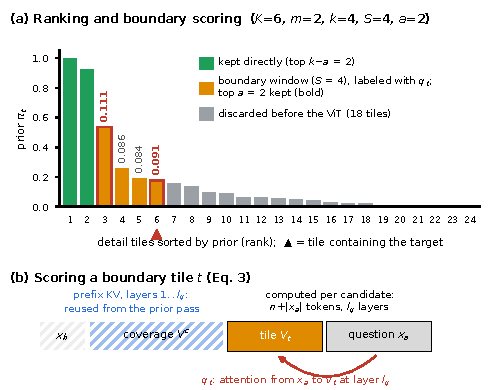
\includegraphics[width=\linewidth]{figures/fig_boundary.pdf}
  \caption{\textbf{Boundary scoring} on the example of \cref{fig:method}. (a) Detail tiles sorted by the
  prior $\pi_t$. The top $k-a$ tiles are kept directly, the next $S$ tiles are scored by question
  attention $q_t$ (\cref{eq:qattn}) and the top $a$ are kept, and the rest are discarded before the
  vision encoder. The target tile is ranked sixth by the prior but has the second-highest $q_t$ in the
  window. (b) Each candidate reuses the prefix KV cache of $[\mathbf{x}_b;\mathbf{V}^c]$ from the prior
  pass, so only $n+|\mathbf{x}_a|$ tokens are processed per tile.}
  \label{fig:boundary}
\end{figure}

% ─────────────────────────────────────────────────────────────────────────────
% Supplementary：從正文 4.5 移出（使用者 2026-10-26 決定正文不放）。表格由 build_paper_results.py 產生（tab_analysis.tex）。
% 由 CVPR27.tex 接在 references 之後 \input。
% ─────────────────────────────────────────────────────────────────────────────
\section{Where \method helps and where it fails}
\label{sec:analysis}

\providecommand{\pend}{\textcolor{red}{?}}

\begin{table}[t]
  \centering
  \footnotesize
  \setlength{\tabcolsep}{2pt}
  \begin{tabular}{l cc cc cc cc}
    \toprule
    & \multicolumn{2}{c}{HR-4K} & \multicolumn{2}{c}{HR-8K} & \multicolumn{4}{c}{V$^*$ Bench} \\
    \cmidrule(lr){2-3}\cmidrule(lr){4-5}\cmidrule(lr){6-9}
    Method & S & C & S & C & Attr. & Pos. & Hit & Miss \\
    \midrule
    Uncompressed & 77.0 & 47.0 & 66.0 & 47.0 & 85.2 & 81.6 & 86.8 & 76.4 \\
    \midrule
    FastV & 73.0 & \textbf{45.0} & 63.0 & \textbf{45.0} & 80.0 & 77.6 & 83.1 & \textbf{69.1} \\
    SparseVLM & 75.0 & 44.0 & 66.0 & 41.0 & 80.0 & \textbf{78.9} & 85.3 & 65.5 \\
    VisionZip & 62.0 & 36.0 & 59.0 & 30.0 & 75.7 & 61.8 & 73.5 & 61.8 \\
    HiRED & 63.0 & 44.0 & 55.0 & 42.0 & 71.3 & 75.0 & 77.9 & 60.0 \\
    IF-Prune & \textbf{76.0} & 39.0 & \textbf{68.0} & 37.0 & \textbf{85.2} & 76.3 & 86.8 & \textbf{69.1} \\
    \rowcolor{oursbg}
    \method (ours) & 71.0 & 42.0 & 61.0 & 43.0 & 77.4 & 77.6 & \textbf{88.2} & 50.9 \\
    \bottomrule
  \end{tabular}
  \caption{\textbf{Where \method helps and where it fails} ($B=1536$). HR-Bench is split into single- (S) and cross-instance (C) questions (CircularEval), V$^*$ Bench into attribute and relative-position questions. Hit / Miss split V$^*$ Bench by whether the detail tiles selected by \method cover the target (136 hit, 55 miss); every method is evaluated on the same split.}
  \label{tab:analysis}
\end{table}


\cref{tab:analysis} breaks down the high-resolution benchmarks by question type. On questions that
involve several objects or the global arrangement of the scene (HR-Bench cross-instance, V$^*$ Bench
relative position), \method is on par with or better than the baselines, \eg 43.0 \vs 37.0 for IF-Prune
on HR-Bench 8K cross-instance. Its gap is concentrated on questions about a single small object
(HR-Bench single-instance, V$^*$ Bench attributes).

V$^*$ Bench provides target boxes, which tell us why. When the selected detail tiles cover the target
(136 of 191 questions), \method answers 88.2\% correctly, on par with the best baseline and the
uncompressed model (86.8\%), since the target is seen at native resolution without the distraction of
the other tiles. When the target is missed, accuracy drops to 50.9\%. The misses come from the prior,
not from boundary scoring: most missed targets are ranked outside the scoring window, while targets
that enter the window are selected 72--94\% of the time, depending on the budget (\cref{tab:window}). The prior is computed
on the coverage tiles, in which more than half of the V$^*$ targets are smaller than one ViT patch
(14\,px), so a small budget can leave them out of the window. Methods
that encode every tile do not have this failure mode, but pay $\mathcal{O}(N)$ for it.


% ─────────────────────────────────────────────────────────────────────────────
% Supplementary: details of Sec. 3.2. tab_recall_full.tex and the numbers here come from paper/figures/make_recall_figure.py
% and results/diagnostics/vstar_selection/ (post-hoc analysis of frozen v1.0, V* Bench only).
% ─────────────────────────────────────────────────────────────────────────────
\section{Details of the reliability analysis}
\label{sec:reliability_supp}

\begin{table}[t]
  \centering
  \footnotesize
  \setlength{\tabcolsep}{4pt}
  \begin{tabular}{lc cc cc}
    \toprule
    $B$ & $K$ & Random & Uniform & Coarse prior & After scoring \\
    \midrule
    1024 & 2 & 7.2 & 3.7 & 27.7 & \textbf{69.1} \\
    1536 & 4 & 14.8 & 8.9 & 67.0 & \textbf{71.2} \\
    2048 & 4 & 14.8 & 8.9 & 59.7 & \textbf{72.8} \\
    3072 & 6 & 22.6 & 14.1 & 77.5 & \textbf{80.1} \\
    \bottomrule
  \end{tabular}
  \caption{\textbf{Recall@$K$ (\%) on V$^*$~Bench} at about the number of detail tiles each budget keeps, with $K$ fixed so that all columns are comparable. Random and uniform selection do not depend on the budget.}
  \label{tab:recall}
\end{table}

\begin{table}[t]
  \centering
  \footnotesize
  \setlength{\tabcolsep}{2.5pt}
  \begin{tabular}{lc ccc cc}
    \toprule
    $B$ & Window & Prior & Recov. & Lost & Final & Rate (rand.) \\
    \midrule
    1024 & 2 of 5 & 53 & +79 & 0 & \textbf{69.1\%} & 89.8\% (33.8\%) \\
    1536 & 2 of 4 & 126 & +17 & $-$7 & \textbf{71.2\%} & 77.3\% (39.4\%) \\
    2048 & 2 of 4 & 115 & +27 & $-$2 & \textbf{73.3\%} & 79.4\% (33.8\%) \\
    3072 & 1 of 3 & 149 & +9 & $-$4 & \textbf{80.6\%} & 64.3\% (31.0\%) \\
    \bottomrule
  \end{tabular}
  \caption{\textbf{From the prior to the final selection} on the 191 questions of V$^*$~Bench. Prior: questions on which the prior alone covers the target with the tiles of the budget. Recov.: the target enters the window, the prior alone would miss it, and boundary scoring keeps it. Lost: the reverse. Final = (prior + recovered $-$ lost) / 191. Rate: the recovery rate, computed over the questions whose target enters the window and that the prior alone would miss (88, 22, 34, 14 questions); in parentheses, the expected rate when the window tiles are kept at random.}
  \label{tab:window}
\end{table}

\begin{table*}[t]
  \centering
  \footnotesize
  \setlength{\tabcolsep}{4pt}
  \begin{tabular}{r cc cc cc cc}
    \toprule
    & \multicolumn{2}{c}{$B=1024$} & \multicolumn{2}{c}{$B=1536$} & \multicolumn{2}{c}{$B=2048$} & \multicolumn{2}{c}{$B=3072$} \\
    \cmidrule(lr){2-3}\cmidrule(lr){4-5}\cmidrule(lr){6-7}\cmidrule(lr){8-9}
    $K$ & Prior & After scoring & Prior & After scoring & Prior & After scoring & Prior & After scoring \\
    \midrule
    1 & 3.1 & 51.3 & 3.1 & 3.1 & 3.1 & 3.1 & 3.1 & 3.1 \\
    2 & 27.7 & 69.1 & 26.7 & 30.4 & 23.6 & 23.6 & 27.7 & 27.7 \\
    3 & 51.3 & 71.2 & 50.3 & 61.3 & 46.1 & 61.8 & 42.9 & 42.9 \\
    4 & 68.6 & 72.8 & 67.0 & 71.2 & 59.7 & 72.8 & 58.1 & 58.1 \\
    5 & 73.8 & 73.8 & 72.8 & 74.3 & 69.1 & 77.0 & 68.1 & 68.1 \\
    6 & 78.5 & 78.5 & 78.5 & 78.5 & 77.5 & 78.0 & 77.5 & 80.1 \\
    8 & 85.3 & 85.3 & 85.9 & 85.9 & 84.3 & 84.3 & 85.3 & 85.3 \\
    12 & 95.3 & 95.3 & 94.8 & 94.8 & 92.1 & 92.1 & 93.2 & 93.2 \\
    \bottomrule
  \end{tabular}
  \caption{\textbf{Recall@$K$ (\%) of the coarse prior and after boundary scoring} on V$^*$~Bench, at every budget with saved selections.}
  \label{tab:recall_full}
\end{table*}


\cref{tab:recall,tab:window} give the numbers behind \cref{sec:reliability}. Little has to be found: of a median of
24 detail tiles, one tile covers the target on 78.5\% of the questions, and two tiles on all of them. Boundary scoring
recovers the targets that the prior alone would miss at 2.0 to 2.7 times the rate of random selection
(\cref{tab:window}).

\cref{tab:recall_full} extends \cref{tab:recall} to all budgets with saved selections. Boundary scoring only
reorders the tiles inside the window, so the two values coincide at every $K$ outside the window. The coverage
view, and thus the prior, changes with the budget because $m=\lfloor K/2\rfloor$. Hits follow the definition of
\cref{sec:reliability}. In this table, the top of the refined ranking consists of the directly kept tiles in
prior order, followed by the window in the order of $q_t$ and the remaining tiles in prior order.

\paragraph{Why the top of the ranking needs a second stage.}
At $B=1536$, the first-ranked tile of the prior is the same as with the neutral question ``Describe this
image.'' on 90.6\% of the questions, and the same as with the swapped question on 91.6\%; the median
correlation between the prior with the real and the neutral question is 0.93. This tile falls into the top
quarter of the image on 63.4\% of the questions (62.3\%, 82.7\%, and 82.2\% at $B=1024$, $2048$, and $3072$), whereas
the top quarter holds the center of a target on only 4.7\% of the questions. The dependence on the question
therefore shows below the first rank, which is where the prior separates from the swapped-question prior
in \cref{fig:recall}. We have not established the cause of this pattern, and we did not change the method in
response to it.

\paragraph{Upper bound of the scorer.}
If $q_t$ is computed for all detail tiles, its first-ranked tile covers the target on 56.5\% of the questions,
and its top $k$ tiles on 84.8\%, against 71.2\% for the selection of \method at $B=1536$. This requires encoding
every tile and thus gives up the bound on compute, so it serves only as a reference. The neutral question
reaches a Recall@5 of 22.0\%, close to a center-first ranking (22.5\%), and the swapped question 49.2\%.

\paragraph{Target size.}
Measured in the coverage tiles at $B=1536$, 63.4\% of the questions have a target whose short side is below one
ViT patch (14\,px). Boundary scoring raises the hit rate from 59.5\% to 66.9\% on these questions, and from 77.1\%
to 78.6\% on the others.

\section{Model scale}
\label{sec:scale}

\providecommand{\pend}{\textcolor{red}{?}}

\begin{table*}[t]
  \centering
  \footnotesize
  \setlength{\tabcolsep}{4.5pt}
  \begin{tabular}{l ccccc c cc}
    \toprule
    Method & DocVQA & InfoVQA & MME-RW & HR-Bench 4K & V$^*$ Bench & Avg.\ (\%) & TTFT (s)$\downarrow$ & Mem.\ (GB)$\downarrow$ \\
    \midrule
    \multicolumn{9}{c}{\textit{InternVL3.5-4B, $B=1536$}} \\
    Uncompressed (score) & 91.0 & 77.6 & 49.5 & 59.5 & 81.2 & 100.0 & 1.24 & 1.81 \\
    FastV & 89.9 & 77.8 & 93.4 & 89.9 & 96.1 & 89.4 & 0.56 & 1.03 \\
    SparseVLM & 62.1 & 79.2 & 94.8 & 89.1 & 97.4 & 84.5 & 0.63 & 1.07 \\
    VisionZip & 51.3 & 49.8 & 65.9 & 52.9 & 74.8 & 59.0 & 0.53 & 0.40 \\
    IF-Prune & \textbf{97.1} & 91.8 & 95.0 & 90.8 & \textbf{98.1} & \textbf{94.6} & 1.05 & 2.70 \\
    \rowcolor{oursbg}
    \method (ours) & 95.1 & \textbf{94.7} & \textbf{95.5} & \textbf{92.4} & 94.8 & 94.5 & \textbf{0.50} & \textbf{0.37} \\
    \midrule
    \multicolumn{9}{c}{\textit{InternVL3.5-8B, $B=1536$}} \\
    Uncompressed (score) & 91.4 & 78.7 & 51.6 & 62.0 & 83.8 & 100.0 & 1.74 & 2.05 \\
    FastV & 91.9 & 77.4 & 90.9 & 95.2 & 94.4 & 90.0 & 0.69 & 1.33 \\
    SparseVLM & 60.3 & 79.1 & 97.4 & \textbf{96.0} & 95.0 & 85.5 & 0.81 & 1.35 \\
    VisionZip & 53.3 & 60.4 & 80.9 & 79.0 & 83.8 & 71.5 & \textbf{0.64} & 0.48 \\
    IF-Prune & \textbf{96.5} & 92.3 & 95.6 & 92.7 & \textbf{97.5} & 94.9 & 1.18 & 2.95 \\
    \rowcolor{oursbg}
    \method (ours) & 95.2 & \textbf{95.0} & \textbf{100.9} & 91.1 & 92.5 & \textbf{95.0} & 0.72 & \textbf{0.41} \\
    \midrule
    \multicolumn{9}{c}{\textit{InternVL3.5-14B, $B=1536$}} \\
    Uncompressed (score) & 92.8 & 80.2 & 52.0 & 61.0 & 84.3 & 100.0 & 2.76 & 2.48 \\
    FastV & 91.4 & 79.6 & 91.2 & 96.7 & \textbf{98.1} & 91.4 & 0.95 & 1.73 \\
    SparseVLM & 64.9 & 76.7 & \textbf{97.5} & 92.6 & 93.8 & 85.1 & 1.14 & 1.76 \\
    VisionZip & 59.9 & 62.7 & 84.4 & 86.9 & 90.1 & 76.8 & \textbf{0.86} & 0.55 \\
    IF-Prune & \textbf{96.9} & 92.7 & 96.6 & 95.1 & 96.9 & \textbf{95.6} & 1.45 & 3.27 \\
    \rowcolor{oursbg}
    \method (ours) & 96.4 & \textbf{94.5} & 96.7 & \textbf{97.5} & 90.7 & 95.2 & 1.11 & \textbf{0.43} \\
    \bottomrule
  \end{tabular}
  \caption{\textbf{Model scale.} Percentage of the uncompressed score at $B=1536$ on InternVL3.5-4B, -8B, and -14B (the uncompressed rows give raw scores). \method uses the hyperparameters calibrated on the 8B model without re-tuning; its attention layers are mapped by relative depth. Best compressed result per model in bold.}
  \label{tab:scale}
\end{table*}


\cref{tab:scale} repeats the default setting on InternVL3.5-4B and \mbox{-14B}, using the hyperparameters
calibrated on the 8B model; only the attention layers are mapped by relative depth. The results
carry over without re-tuning. On all three models, \method is among the two most accurate methods
(94.5\%, 95.0\%, and 95.2\%), well ahead of FastV (89.4 to 91.4), SparseVLM (84.5 to 85.5), HiRED (70.5 to 81.2), and
VisionZip (59.0 to 76.8). The memory advantage holds at every scale: \method uses the least memory on all three models
(0.37, 0.41, and 0.43\,GB), since its footprint is set by the budget and not by the input, whereas
IF-Prune needs 2.70 to 3.27\,GB, about 7$\times$ more, and FastV and SparseVLM over 1\,GB. \method is
also faster than IF-Prune on every model (2.1$\times$ on 4B, 1.3$\times$ on 14B), and on 4B it is the
fastest of all methods (0.50\,s). On InfoVQA, \method remains the best method on every model, and on
HR-Bench 4K it is the best on 4B and 14B.

% ─────────────────────────────────────────────────────────────────────────────
% Supplementary: same-budget downscaling (docs/06 §9 #2). Tables from results/paper/build_downscale_tables.py.
% ─────────────────────────────────────────────────────────────────────────────
\section{Same-budget downscaling}
\label{sec:supp_downscale}

\begin{table}[t]
  \centering
  \footnotesize
  \setlength{\tabcolsep}{3.4pt}
  \begin{tabular}{l cc cc cc}
    \toprule
    & \multicolumn{2}{c}{$B=1536$} & \multicolumn{2}{c}{$B=2560$} & \multicolumn{2}{c}{$B=3072$} \\
    \cmidrule(lr){2-3}\cmidrule(lr){4-5}\cmidrule(lr){6-7}
    Method & Avg. & Small & Avg. & Small & Avg. & Small \\
    \midrule
    Low-Res & 84.2 & 73.5 & 92.9 & 85.4 & 93.3 & 85.9 \\
    Low-Res-Fill & 91.7 & 82.6 & 94.1 & 86.6 & 96.2 & 90.3 \\
    \rowcolor{oursbg}
    \method (ours) & \textbf{95.0} & \textbf{91.9} & \textbf{97.6} & \textbf{93.8} & \textbf{99.3} & \textbf{95.5} \\
    \bottomrule
  \end{tabular}
  \caption{\textbf{Same-budget downscaling}, as a percentage of the uncompressed score. Avg.: the five benchmarks of \cref{tab:main}; Small: HR-Bench 4K, HR-Bench 8K, and V$^*$. Low-Res is the official tiling capped at $K=B/256$ tiles, which cannot always fill the budget (on average 1{,}149/1{,}931/1{,}972 visual tokens); Low-Res-Fill gives the whole budget to coverage tiles ($m{=}K$). Per-benchmark scores and paired confidence intervals are in the supplementary material.}
  \label{tab:downscale}
\end{table}

\begin{table*}[t]
  \centering
  \footnotesize
  \setlength{\tabcolsep}{4pt}
  \begin{tabular}{l c ccc ccc ccc}
    \toprule
    & & \multicolumn{3}{c}{$B=1536$} & \multicolumn{3}{c}{$B=2560$} & \multicolumn{3}{c}{$B=3072$} \\
    \cmidrule(lr){3-5}\cmidrule(lr){6-8}\cmidrule(lr){9-11}
    Benchmark & Unc. & Low-Res & Fill & Ours & Low-Res & Fill & Ours & Low-Res & Fill & Ours \\
    \midrule
    DocVQA & 91.4 & 85.3 & \textbf{89.8} & 87.0 & 90.0 & 89.8 & \textbf{90.1} & 90.1 & \textbf{91.2} & 90.3 \\
    InfoVQA & 78.7 & 67.3 & 73.6 & \textbf{74.8} & 73.2 & 77.8 & \textbf{78.6} & 74.0 & 78.8 & \textbf{79.4} \\
    MME-RW & 51.6 & 45.5 & 49.9 & \textbf{52.1} & 50.2 & 49.9 & \textbf{52.2} & 50.2 & 51.0 & \textbf{53.5} \\
    HR-4K & 62.0 & 47.5 & 51.5 & \textbf{56.5} & 55.0 & 54.5 & \textbf{58.0} & 55.5 & 56.5 & \textbf{59.5} \\
    V$^*$ & 83.8 & 64.9 & 72.8 & \textbf{77.5} & 72.8 & 74.3 & \textbf{79.6} & 72.8 & 76.4 & \textbf{81.7} \\
    HR-8K & 56.5 & 37.5 & 44.0 & \textbf{52.0} & 45.5 & 47.0 & \textbf{52.5} & 46.0 & 50.0 & \textbf{52.5} \\
    \midrule
    Low-Res tokens & -- & \multicolumn{3}{c}{1{,}149 / 1{,}536} & \multicolumn{3}{c}{1{,}931 / 2{,}560} & \multicolumn{3}{c}{1{,}972 / 3{,}072} \\
    \bottomrule
  \end{tabular}
  \caption{\textbf{Same-budget downscaling: scores.} Fill: Low-Res-Fill ($m{=}K$). Low-Res tokens: average number of visual tokens used by Low-Res over the five benchmarks of \cref{tab:main}, against the budget; Low-Res-Fill and \method use exactly $B$.}
  \label{tab:downscale_full}
\end{table*}

\begin{table*}[t]
  \centering
  \scriptsize
  \setlength{\tabcolsep}{2.4pt}
  \begin{tabular}{l cc cc cc}
    \toprule
    & \multicolumn{2}{c}{$B=1536$} & \multicolumn{2}{c}{$B=2560$} & \multicolumn{2}{c}{$B=3072$} \\
    \cmidrule(lr){2-3}\cmidrule(lr){4-5}\cmidrule(lr){6-7}
    Benchmark & vs.\ Fill & vs.\ Low-Res & vs.\ Fill & vs.\ Low-Res & vs.\ Fill & vs.\ Low-Res \\
    \midrule
    DocVQA & $-$2.7\,[$-$3.6,\,$-$1.9] & \textbf{+1.7\,[+0.8,\,+2.6]} & +0.3\,[$-$0.5,\,+1.0] & +0.1\,[$-$0.6,\,+0.8] & $-$0.9\,[$-$1.5,\,$-$0.2] & +0.2\,[$-$0.5,\,+0.8] \\
    InfoVQA & +1.2\,[$-$0.3,\,+2.6] & \textbf{+7.6\,[+6.1,\,+9.1]} & +0.8\,[$-$0.5,\,+2.1] & \textbf{+5.4\,[+4.0,\,+6.8]} & +0.6\,[$-$0.7,\,+1.7] & \textbf{+5.3\,[+4.0,\,+6.6]} \\
    MME-RW & \textbf{+2.2\,[+0.4,\,+4.0]} & \textbf{+6.6\,[+4.7,\,+8.4]} & \textbf{+2.3\,[+0.6,\,+3.9]} & \textbf{+1.9\,[+0.2,\,+3.8]} & \textbf{+2.5\,[+0.9,\,+4.1]} & \textbf{+3.2\,[+1.5,\,+5.0]} \\
    HR-4K & +5.0\,[$-$1.5,\,+12.0] & \textbf{+9.0\,[+2.5,\,+15.5]} & +3.5\,[$-$2.0,\,+9.5] & +3.0\,[$-$2.5,\,+8.5] & +3.0\,[$-$3.0,\,+8.5] & +4.0\,[$-$1.5,\,+9.0] \\
    V$^*$ & +4.7\,[$-$1.0,\,+11.0] & \textbf{+12.6\,[+5.2,\,+19.9]} & +5.2\,[$-$1.0,\,+12.0] & \textbf{+6.8\,[+1.0,\,+13.1]} & +5.2\,[$-$0.5,\,+11.5] & \textbf{+8.9\,[+2.6,\,+15.2]} \\
    HR-8K & \textbf{+8.0\,[+0.5,\,+15.0]} & \textbf{+14.5\,[+7.5,\,+22.0]} & +5.5\,[$-$1.0,\,+12.0] & +7.0\,[+0.0,\,+13.5] & +2.5\,[$-$3.0,\,+8.0] & +6.5\,[+0.0,\,+12.5] \\
    \bottomrule
  \end{tabular}
  \caption{\textbf{Same-budget downscaling: paired differences} (\method minus baseline, points) with 95\% paired bootstrap intervals (2{,}000 resamples; HR-Bench resamples CircularEval groups). Bold: the interval excludes zero in favor of \method.}
  \label{tab:downscale_delta}
\end{table*}


\paragraph{Baselines.}
Both baselines use InternVL3.5-8B with the prompts, decoding, and evaluation of \cref{sec:main}, on the full test
sets, at $B\in\{1536,2560,3072\}$ with $K=B/256$. \emph{Low-Res} is the official dynamic tiling with the tile cap
set to $K$ and the thumbnail added as usual, and no compression afterwards. It is the standard way to run InternVL
at a lower resolution, but the official aspect-ratio grid often cannot use all $K$ tiles, so it uses fewer visual
tokens than the budget on average (\cref{tab:downscale_full}). At $B=2560$, the grid plus thumbnail exceeds the
budget by one tile on 41 of 11{,}860 questions. \emph{Low-Res-Fill} is \method with $m=K$: the whole budget goes to
coverage tiles of the downscaled image, no detail tile is selected, and it uses exactly $B$ visual tokens. It is
the coverage-only variant of \cref{tab:ablation}, evaluated on the test sets.

\paragraph{Results.}
\cref{tab:downscale_delta} gives the paired differences. \method is significantly better than Low-Res on InfoVQA,
MME-RealWorld, and V$^*$ Bench at every budget, and on all six benchmarks at $B=1536$. Against Low-Res-Fill, it is
ahead on all three small-object benchmarks at every budget, by 2.5 to 8.0 points, and significantly better on
MME-RealWorld at every budget and on HR-Bench 8K at $B=1536$.

% ─────────────────────────────────────────────────────────────────────────────
% Supplementary: TTFT breakdown (docs/06 §9 #6). Table from results/paper/build_ttft_breakdown.py,
% using the existing efficiency measurements (no extra runs).
% ─────────────────────────────────────────────────────────────────────────────
\section{TTFT breakdown}
\label{sec:supp_ttft}

% 由 results/paper/build_ttft_breakdown.py 產生，不要手改
\begin{table*}[t]
  \centering
  \small
  \setlength{\tabcolsep}{4.5pt}
  \begin{tabular}{lccccccccccc}
    \toprule
    & \multicolumn{5}{c}{(a) Budget $B$ (five benchmarks)} & & \multicolumn{5}{c}{(b) Input tiles (HR-8K)} \\
    \cmidrule(lr){2-6}\cmidrule(lr){8-12}
    Stage (ms) & 1024 & 1536 & 2048 & 2560 & 3072 & & 7 & 25 & 78 & 127 & 188 \\
    \midrule
    Prefill of $\mathbf{x}_b$ & 41 & 41 & 41 & 41 & 41 & & 41 & 41 & 42 & 42 & 43 \\
    Vision encoder, coverage tiles & 20 & 22 & 41 & 43 & 65 & & 22 & 22 & 23 & 24 & 23 \\
    Prior pass & 95 & 101 & 174 & 180 & 246 & & 98 & 99 & 99 & 100 & 99 \\
    Vision encoder, detail tiles & 62 & 70 & 69 & 86 & 88 & & 68 & 70 & 70 & 71 & 72 \\
    Boundary scoring ($q_t$) & 172 & 140 & 149 & 118 & 124 & & 129 & 131 & 137 & 132 & 136 \\
    Prefill of selected tiles & 188 & 290 & 381 & 488 & 580 & & 288 & 291 & 291 & 294 & 292 \\
    Prefill of $\mathbf{x}_a$ + first token & 42 & 42 & 43 & 43 & 44 & & 42 & 42 & 42 & 42 & 42 \\
    \midrule
    \rowcolor{oursbg}
    TTFT, \method & 623 & 709 & 899 & 1002 & 1191 & & 690 & 699 & 706 & 707 & 710 \\
    \quad of which selection (prior + $q_t$) & 43\% & 34\% & 36\% & 30\% & 31\% & & 33\% & 33\% & 33\% & 33\% & 33\% \\
    TTFT, uncompressed & \multicolumn{5}{c}{1740 (independent of $B$)} & & 414 & 1428 & 5258 & 10013 & 17229 \\
    \bottomrule
  \end{tabular}
  \caption{\textbf{TTFT breakdown} of \method on InternVL3.5-8B (mean in ms; the stages add up to the mean TTFT up to about 2\,ms of CPU time). (a) Mean over DocVQA, InfoVQA, MME-RealWorld, HR-Bench 4K, and V$^*$ Bench, 50 images each. (b) HR-Bench 8K with the tile cap raised from 7 to 201, at $B=1536$; columns give the mean number of input tiles including the thumbnail.}
  \label{tab:ttft}
\end{table*}


\cref{tab:ttft} splits the TTFT of \method into the stages of \cref{alg:foveatile}, measured as in
\cref{sec:setup}. The two stages that exist only to select tiles, the prior pass and boundary scoring, take
240 to 270\,ms at $B\le1536$ and 300 to 370\,ms at larger budgets. They replace the encoding and prefill
of the tiles that are never selected.

\paragraph{Budget.} The largest stage is the prefill of the selected tiles, which grows linearly with $B$
(188 to 580\,ms). The prior pass grows with the $m=\lfloor K/2\rfloor$ coverage tiles it reads, and boundary
scoring shrinks as the window $S$ narrows from 5 to 3. The text prefills before and after the image take
about 40\,ms each at every budget.

\paragraph{Resolution.} Raising the tile cap from 7 to 201 changes no stage by more than 10\,ms, and TTFT
stays between 0.69 and 0.71\,s, as \cref{tab:complexity} predicts: every stage depends on $K$ and $S$ and
none on $N$. The detail tiles that fall outside the directly kept set and the window are never encoded,
so the vision encoder runs on the same number of tiles at every resolution. Without compression, TTFT grows
from 1.4\,s at 25 tiles to 17.2\,s at 188 tiles, 24$\times$ the TTFT of \method.

% ─────────────────────────────────────────────────────────────────────────────
% Supplementary: calibration protocol. Condensed from docs/04_calibration_protocol.md (full record, every number from there).
% ─────────────────────────────────────────────────────────────────────────────
\section{Calibration protocol}
\label{sec:calibration}

Apart from the attention layers, all hyperparameters of \method were set on two held-out calibration sets. Apart from choosing those layers, the test sets were used only to report results and to diagnose errors; any change suggested by a diagnosis had to pass on the calibration sets first.

\paragraph{Calibration sets.}
\emph{InfoVQA train} consists of 600 questions sampled with a fixed seed from the train split (ANLS).
\emph{MME-RW calib} is drawn from the full English MME-RealWorld (23,609 questions): we remove the questions of
the Lite subset (1,787) and all other questions on its images (2,654), and sample 120 of the remaining 19,168
questions from each of the five subtasks (accuracy, 600 questions). The result shares no questions and no images with the Lite test set.
DocVQA has no train split with answers, so InfoVQA train also represents documents.

\paragraph{Metrics.}
Retention is the score divided by the uncompressed score on the same set (83.9 and 59.5). We report its average
over the two sets and its worst value over six groups (InfoVQA and the five subtasks). TTFT is the median over 50
images after one warm-up image, with one process per GPU. Comparisons use a paired bootstrap on the same questions
with 2,000 resamples (4,000 in the candidate tests) at 95\% confidence.

\begin{table}[t]
  \centering
  \footnotesize
  \setlength{\tabcolsep}{4pt}
  \begin{tabular}{l ccccc c}
    \toprule
    $m$ & 1024 & 1536 & 2048 & 2560 & 3072 & Mean \\
    \midrule
    $1$ & 57.9 & 61.2 & 63.9 & 65.2 & 68.4 & 63.3 \\
    $K/2$ & 63.9 & 68.4 & 68.8 & 70.7 & 71.0 & \textbf{68.5} \\
    $3K/4$ & 65.2 & 67.6 & 68.3 & 70.0 & 70.9 & 68.4 \\
    $K$ & 63.5 & 68.8 & 69.1 & 70.1 & 71.8 & 68.6 \\
    \bottomrule
  \end{tabular}
  \caption{\textbf{Stage A: coverage fraction.} Score averaged over the two calibration sets, per budget $B$.}
  \label{tab:calib_m}
\end{table}

\begin{table}[t]
  \centering
  \footnotesize
  \setlength{\tabcolsep}{2pt}
  \begin{tabular}{l ccc ccc ccc}
    \toprule
    & \multicolumn{3}{c}{$m=K/2$} & \multicolumn{3}{c}{$m=3K/4$} & \multicolumn{3}{c}{$m=K$} \\
    \cmidrule(lr){2-4}\cmidrule(lr){5-7}\cmidrule(lr){8-10}
    $B$ & Avg. & Min & TTFT & Avg. & Min & TTFT & Avg. & Min & TTFT \\
    \midrule
    1024 & 89.7 & 76 & 0.90 & 91.2 & 77 & 0.69 & 88.5 & 80 & 0.40 \\
    1536 & 95.7 & 85 & 0.99 & 94.3 & 72 & 0.89 & 96.2 & 86 & 0.45 \\
    2048 & 95.9 & 85 & 1.08 & 95.5 & 72 & 1.00 & 96.0 & 74 & 0.56 \\
    2560 & 98.9 & 94 & 1.19 & 97.9 & 82 & 1.15 & 97.7 & 69 & 0.69 \\
    3072 & 99.3 & 86 & 1.41 & 99.1 & 83 & 1.32 & 100.1 & 78 & 0.80 \\
    \bottomrule
  \end{tabular}
  \caption{\textbf{Retention (\%) and TTFT (s)} for the three plausible coverage fractions, before the window was calibrated. Avg.: average over the two sets. Min: worst of the six groups.}
  \label{tab:calib_ret}
\end{table}

\paragraph{Stage A: coverage fraction and default budget.}
We swept $m\in\{1,K/4,K/2,3K/4,K\}$ with a provisional window. Using only the thumbnail ($m=1$) loses about 5
points at every budget (\cref{tab:calib_m}), while $m/K$ from 0.5 to 1 forms a plateau whose differences are mostly not significant.
Since the averages tie, we chose by stability: $m=K/2$ has the most stable worst-group retention (\cref{tab:calib_ret}). We set
$B=1536$ as the default because retention saturates there (90\% at $B=1024$, 96\% at $B=1536$, no further gain at $B=2048$).
Pure coverage ($m=K$) is about twice as fast and is reported as an ablation.

\begin{table*}[t]
  \centering
  \footnotesize
  \setlength{\tabcolsep}{4pt}
  \begin{tabular}{l c c c c}
    \toprule
    $B$ & $S$ & Avg.\ retention (\%) & Worst group (\%) & TTFT (s) \\
    \midrule
    1024 & 0 / \textbf{5} / 10 / 15 / 20 & 85.9 / \textbf{89.6} / 89.7 / 88.6 / 89.3 & 61.5 / \textbf{77.7} / 75.5 / 73.8 / 73.8 & 0.43 / \textbf{0.67} / 0.89 / 1.12 / 1.35 \\
    1536 & 0 / \textbf{4} / 9 / 13 / 18 & 93.2 / \textbf{95.6} / 95.7 / 95.5 / 94.5 & 80.0 / \textbf{85.1} / 84.6 / 89.2 / 78.5 & 0.58 / \textbf{0.77} / 0.99 / 1.18 / 1.41 \\
    2048 & 0 / \textbf{4} / 8 / 12 / 16 & 95.1 / \textbf{96.7} / 95.9 / 95.5 / 96.2 & 75.4 / \textbf{84.6} / 84.6 / 81.5 / 83.1 & 0.72 / \textbf{0.92} / 1.08 / 1.26 / 1.45 \\
    2560 & 0 / \textbf{3} / 7 / 10 / 14 & 97.7 / \textbf{98.8} / 98.9 / 97.5 / 97.5 & 89.2 / \textbf{93.6} / 93.8 / 83.1 / 80.0 & 0.86 / \textbf{1.02} / 1.19 / 1.30 / 1.48 \\
    3072 & 0 / \textbf{3} / 7 / 10 / 14 & 98.5 / \textbf{98.2} / 99.3 / 98.3 / 100.3 & 86.2 / \textbf{86.2} / 86.2 / 86.2 / 89.2 & 1.05 / \textbf{1.23} / 1.41 / 1.53 / 1.72 \\
    \bottomrule
  \end{tabular}
  \caption{\textbf{Stage B: scoring window} with $m=\lfloor K/2\rfloor$. The adopted value of $S$ is in bold.}
  \label{tab:calib_s}
\end{table*}

\paragraph{Stage B: scoring window.}
We fixed $m=\lfloor K/2\rfloor$ and swept $S\in\{0,S_0/2,S_0,1.5S_0,2S_0\}$, where $S_0$ is the provisional window
(\cref{tab:calib_s}). Removing the window ($S=0$) is significantly worse on local-detail questions, \eg $-$10.8
points [$-$18, $-$4] on Remote Sensing at $B=1024$ and $1536$. Larger windows bring no reliable gain and add TTFT.

\paragraph{Attention layers.}
The layers $\mathcal{L}_p=\{21,\dots,28\}$ and $l_q=20$ were chosen on InfoVQA val before this protocol existed, and
InfoVQA val is also a test set. They were not re-selected on the calibration sets. For the 4B and 14B models they are mapped by
relative depth, by a rule fixed before those models were run.

\begin{table}[t]
  \centering
  \footnotesize
  \setlength{\tabcolsep}{3pt}
  \begin{tabular}{>{\raggedright\arraybackslash}p{0.33\linewidth} >{\raggedright\arraybackslash}p{0.57\linewidth}}
    \toprule
    Candidate & Result on the calibration sets \\
    \midrule
    Window grows with the grid & No $f\in\{0.2,\dots,0.5\}$ passes all criteria; local-detail $\Delta$ at $f=0.2$: +0.67 [$-$0.44, +1.78] \\
    Question-stem query, top-patch aggregation & Worse on local detail for all eight variants, \eg $-$3.33 for the stem query \\
    Options sorted before scoring & Local detail $-$0.19 [$-$0.93, +0.46]; retention $-$0.56 at $B=1536$, misses the limit of $-$0.5 \\
    Attention-head selection, question-free correction & Recall +4.2 on a synthetic set, but retention $-$1.60, $-$0.83, $-$0.85; local detail $-$2.22 [$-$4.35, $-$0.09] \\
    \bottomrule
  \end{tabular}
  \caption{\textbf{Rejected candidates.} All were tested with the criteria below, and each decision used only the calibration sets.}
  \label{tab:calib_rej}
\end{table}

\paragraph{Rejected candidates.}
Diagnosing errors on the test sets suggested the four changes in \cref{tab:calib_rej}. Before each test we fixed three
criteria: average retention at most 0.5 points below the frozen configuration at every budget, a significant gain on the
local-detail questions of MME-RW (Remote Sensing, Monitoring, Autonomous Driving; 360 questions), and at most
0.3\,s of added TTFT at $B=1536$. None of the candidates passed its criteria, so we kept the configuration as frozen.

\paragraph{Deviations from the pre-registered rules.}
\begin{enumerate}
  \item The rule for Stage B selected $S=\{5,13,4,3,14\}$: the smallest $S$ within one point of the best average and
        worst-group retention. Each MME-RW group has only 120 questions, so the rule was driven by noise, and the
        differences to $S_0/2$ are not significant. We therefore used $S_0/2$ at every budget.
  \item The sweep of the growing window added $f=0.2$, since larger $f$ is very costly on MME-RW. The criteria did not change.
  \item Sorted options were added after the results of the other query variants were known. The criteria did not change, and the candidate was rejected.
  \item An earlier configuration had its window table and coverage fraction tuned on test data. We discarded it and
        recalibrated as described here.
\end{enumerate}

% ─────────────────────────────────────────────────────────────────────────────
% Supplementary: baseline ports. Matches the header notes of fastv/sparsevlm/visionzip/ifprune_internvl.py and run_test_suite.sh.
% ─────────────────────────────────────────────────────────────────────────────
\section{Baseline implementation}
\label{sec:baselines}

We ported each baseline to InternVL3.5 from its official code and kept the selection algorithm and official
hyperparameters. All methods share the prompts, the tiling, the greedy decoding, and the measurement code. Budget
$B$ always means the number of visual tokens left in the KV cache, so a method keeps $\min(B,\text{all tokens})$.
The points below are the only decisions that the official code does not determine.

\paragraph{FastV~\cite{fastv}.}
We follow the official in-place variant: at layer 2, the attention of the last token ranks the visual tokens, the top
$B$ are kept, and the sequence is actually shortened, with the original position ids retained. The official in-place
code does not support a KV cache, so we added multi-token decoding with per-layer cache lengths. The pruning
decision is unchanged.

\paragraph{SparseVLM~\cite{sparsevlm}.}
We implement the rank-based removal of the paper at the official relative depths (layers 2, 6, and 15 of 32, scaled
to the depth of the model). The paper publishes no value of $\lambda$, so for each benchmark and budget we search the
smallest $\lambda$ for which the three stages alone reach between $B$ and $1.5B$ tokens, and use the median over 32
images. This step uses only token counts, not answers; images that need no compression are excluded. Remaining
excess tokens are clipped at the final stage. An image with at most $B$ tokens is not pruned ($\lambda=0$), as for
all other methods; the official experiments use a fixed input that always exceeds the budget, so the official code has
no such case.

\paragraph{VisionZip~\cite{visionzip}.}
Dominant and contextual tokens are computed per tile in the feature layer of the vision encoder. The contextual
share of 5/32 reproduces all pairs in the tables of the paper, and we apply it to other sizes as well. The official API
takes the numbers per crop, so we split $B$ evenly over the tiles. InternVL merges $2\times2$ patches by pixel shuffle before the
projector, so tokens are selected and merged after pixel shuffle and before the projector, averaging scores and keys in
each group as in the official Qwen2.5-VL code. The CLS token serves only as the query, since InternVL drops it.

\paragraph{IF-Prune~\cite{ifprune}.}
We load the released guide model (InternVL2.5-1B with its LoRA and importance head) without retraining. It runs once on
all tiles and the question, as in the official evaluation code, and the main model keeps the top $B$ tokens at layer
2, which corresponds to a keep ratio of $B$ divided by the number of tokens. Prefill and decoding follow our FastV
path. The official experiments use InternVL2 main models, so applying the guide to InternVL3.5 is an extrapolation of
their cross-model result. Both models produce 256 tokens per tile in the same order. Memory and TTFT include the guide model.


\end{document}
